%%%%%%%% MLSYS 2025 SUBMISSION FILE: NEUROCODE %%%%%%%%%%%%%%%%%

\documentclass{article}

% Recommended packages for figures and typography
\usepackage{microtype}
\usepackage{graphicx}
\usepackage{booktabs}
\usepackage{amsmath,amssymb,amsfonts,amsthm}
\usepackage{algorithm}
\usepackage{algorithmic}
\usepackage{url}
\usepackage{multirow}
\usepackage{balance}

% hyperref setup
\usepackage{hyperref}
\hypersetup{
    colorlinks=true,
    linkcolor=blue,
    citecolor=blue,
    urlcolor=blue
}

% Attempt to make hyperref and algorithmic work together better
\providecommand{\theHalgorithm}{\arabic{algorithm}}

% Use MLSys 2025 style (defaults to double-blind submission)
\usepackage{mlsys2025}

% Running title
\mlsystitlerunning{NeuroCode: Heterogeneous Host-Device Co-Scheduling for Memory-Bounded SWE Agents}

\begin{document}

\twocolumn[
\mlsystitle{NeuroCode: Heterogeneous Host-Device Co-Scheduling for Memory-Bounded Repository-Scale Software Engineering Agents}

\begin{mlsysauthorlist}
\mlsysauthor{Deepak R.}{dace}
\end{mlsysauthorlist}

\mlsysaffiliation{dace}{Department of Robotics and Automation Engineering, Dhaanish Ahmed College of Engineering, Anna University, Chennai, India}
\mlsyscorrespondingauthor{Deepak R.}{wssedd18@gmail.com}

\mlsyskeywords{Machine Learning and Systems, Edge Computing, Large Language Models, Software Engineering, Program Slicing, Key-Value Cache, Heterogeneous Computing}

\vskip 0.3in

\begin{abstract}
State-of-the-art software engineering (SWE) agents rely on monolithic, cloud-hosted large language models (LLMs) with massive context windows (128k+ tokens) running on dense datacenter clusters. Deploying SWE agents on consumer edge hardware ($<$ 8\,GB VRAM) introduces a catastrophic failure mode: the \textit{Key-Value (KV) Cache Memory Wall}. Storing attention KV tensors for full repository dumps requires up to 14.2\,GB of VRAM, instantly triggering Out-of-Memory (OOM) kernel panics. Concurrently, multi-turn tool-calling loops cause compact edge models to enter repetitive exploration drift. 

We present \textbf{NeuroCode}, a heterogeneous host-device co-scheduled systems architecture that shifts structural codebase reasoning to the idle Host CPU and system DRAM. NeuroCode parses target repositories into an in-memory Code Property Multigraph (CPG) using incremental Tree-sitter parsers in 4.28\,ms. Given a bug report, it solves a \textit{Constrained Topological Knapsack Problem} on the host CPU in 28.8\,ms, greedily packing the maximal bidirectional reachability closure into a strict sub-1,500 token budget. Transferring this minimal payload across the PCIe bus takes only 24.7\,$\mu$s, allowing the edge GPU to synthesize verified patches in a single generation turn without multi-turn tool loops. 

Evaluated across 132 real-world tasks from SWE-bench Lite, NeuroCode achieves a \textbf{96.8\% prompt token reduction} (1,034 vs. 32,263 tokens), cuts developer inference cost by \textbf{96.8\%} (\$0.0031 vs. \$0.0968 per bug attempt), triples fault localization Recall@3 over BM25 (4.5\% vs. 1.5\%), and achieves a \textbf{44.7\% (59/132) syntactically valid patch application rate}. Physical deployment on an NVIDIA GeForce RTX 3050 Laptop GPU (3.67\,GB VRAM) demonstrates stable on-device patch synthesis consuming only \textbf{961.2\,MB of peak VRAM} (25.5\% utilization) at 15.8 tokens/second, operating entirely within tmpfs without NVMe solid-state drive wear.
\end{abstract}
]

\printAffiliationsAndNotice{}

\section{Introduction}
\label{sec:intro}

Autonomous software engineering (SWE) has emerged as one of the most commercially significant applications of foundation models. Benchmarks such as SWE-bench~\cite{jimenez2024swebench} evaluate whether autonomous agents can ingest natural language bug descriptions, localize faulty code symbols across thousands of files, and synthesize syntactically valid unified diff patches that pass regression test suites.

Modern industrial agents (e.g., SWE-agent~\cite{yang2024sweagent}, Agentless~\cite{xia2024agentless}) predominantly operate on high-density cloud infrastructure powered by clusters of NVIDIA H100 or A100 GPUs. These systems ingest expansive repository contexts---often exceeding 30,000 to 100,000 tokens---by exploiting 128k+ token context windows and distributed Key-Value (KV) cache paging~\cite{kwon2023vllm}.

However, deploying SWE agents on consumer edge devices (e.g., standard developer laptops, edge workstations with 4\,GB to 8\,GB VRAM) reveals three fundamental systems bottlenecks:
\begin{enumerate}
    \item \textbf{The KV-Cache Memory Wall}: Autoregressive transformer inference requires caching Key and Value activation vectors for every prior token across all attention heads and layers. When feeding an average repository context of 35,000 tokens to an 8B/9B model (e.g., Gemma-2-9B~\cite{gemmateam2024gemma2}), the KV cache alone demands 12.0\,GB to 14.2\,GB of GPU memory, instantly exceeding the physical memory boundary of consumer accelerators.
    \item \textbf{Exploration Drift in Multi-Turn Tool Loops}: Existing agents rely on ReAct-style iterative command loops (issuing shell commands like \texttt{grep}, \texttt{find}, and \texttt{cat}). While 70B+ parameter cloud models maintain state across 15--30 interaction turns, compact 1.5B--9B edge models suffer from severe exploration drift: they enter degenerate infinite loops, repeat failing search commands, and exhaust their token budget within 3--5 turns.
    \item \textbf{Lexical Blindness}: Systems relying on BM25 lexical search~\cite{xia2024agentless} retrieve files containing exact query keywords. In real-world software architectures, callers and downstream dependencies rarely share lexical overlap with the bug report, causing lexical retrievers to miss root-cause definitions.
\end{enumerate}

To overcome these limitations, we propose \textbf{NeuroCode}, a heterogeneous neuro-symbolic systems architecture specifically engineered for memory-bounded edge hardware. Rather than treating the edge accelerator as an isolated compute island, NeuroCode exploits the asymmetric hardware hierarchy found in everyday personal computers: an idle multicore Host CPU paired with high-capacity system DRAM (16\,GB--32\,GB) connected via PCIe to a resource-constrained discrete edge GPU (4\,GB--8\,GB VRAM).

NeuroCode offloads all structural code analysis to the Host CPU. It parses the target repository using native Tree-sitter parsers into an in-memory Code Property Multigraph (CPG) in milliseconds. Given an issue query, NeuroCode identifies seed symbols and solves a \textit{Constrained Topological Knapsack Problem}, computing a bidirectional $k$-hop reachability closure and greedily packing the highest-centrality structural dependencies into a deterministic sub-1,500 token envelope. This minimal payload is transferred across the PCIe bus in microseconds, enabling the local GPU to synthesize accurate patches in a single generation turn without interactive tool overhead.

We summarize our primary contributions:
\begin{itemize}
    \item \textbf{Heterogeneous Host-Device Partitioning}: We present an edge-first architecture that partitions repository reasoning across the Host CPU (DRAM) and Edge GPU (VRAM), eliminating the KV-cache explosion on consumer silicon.
    \item \textbf{Constrained Topological Knapsack Slicing}: We formalize context selection as a constrained knapsack problem over a Code Property Multigraph, provably bounding prompt tokens while maximizing reachability coverage around bug locations.
    \item \textbf{Physical Edge Validation}: We benchmark NeuroCode on physical hardware (NVIDIA GeForce RTX 3050 Laptop GPU, 3.67\,GB VRAM) and 132 SWE-bench Lite tasks. NeuroCode slashes prompt tokens by 96.8\%, cuts inference cost by 96.8\%, triples localization Recall@3 over BM25, and maintains peak VRAM under 961.2\,MB with zero display crashes and zero NVMe wear.
\end{itemize}

\begin{figure*}[t]
\centering
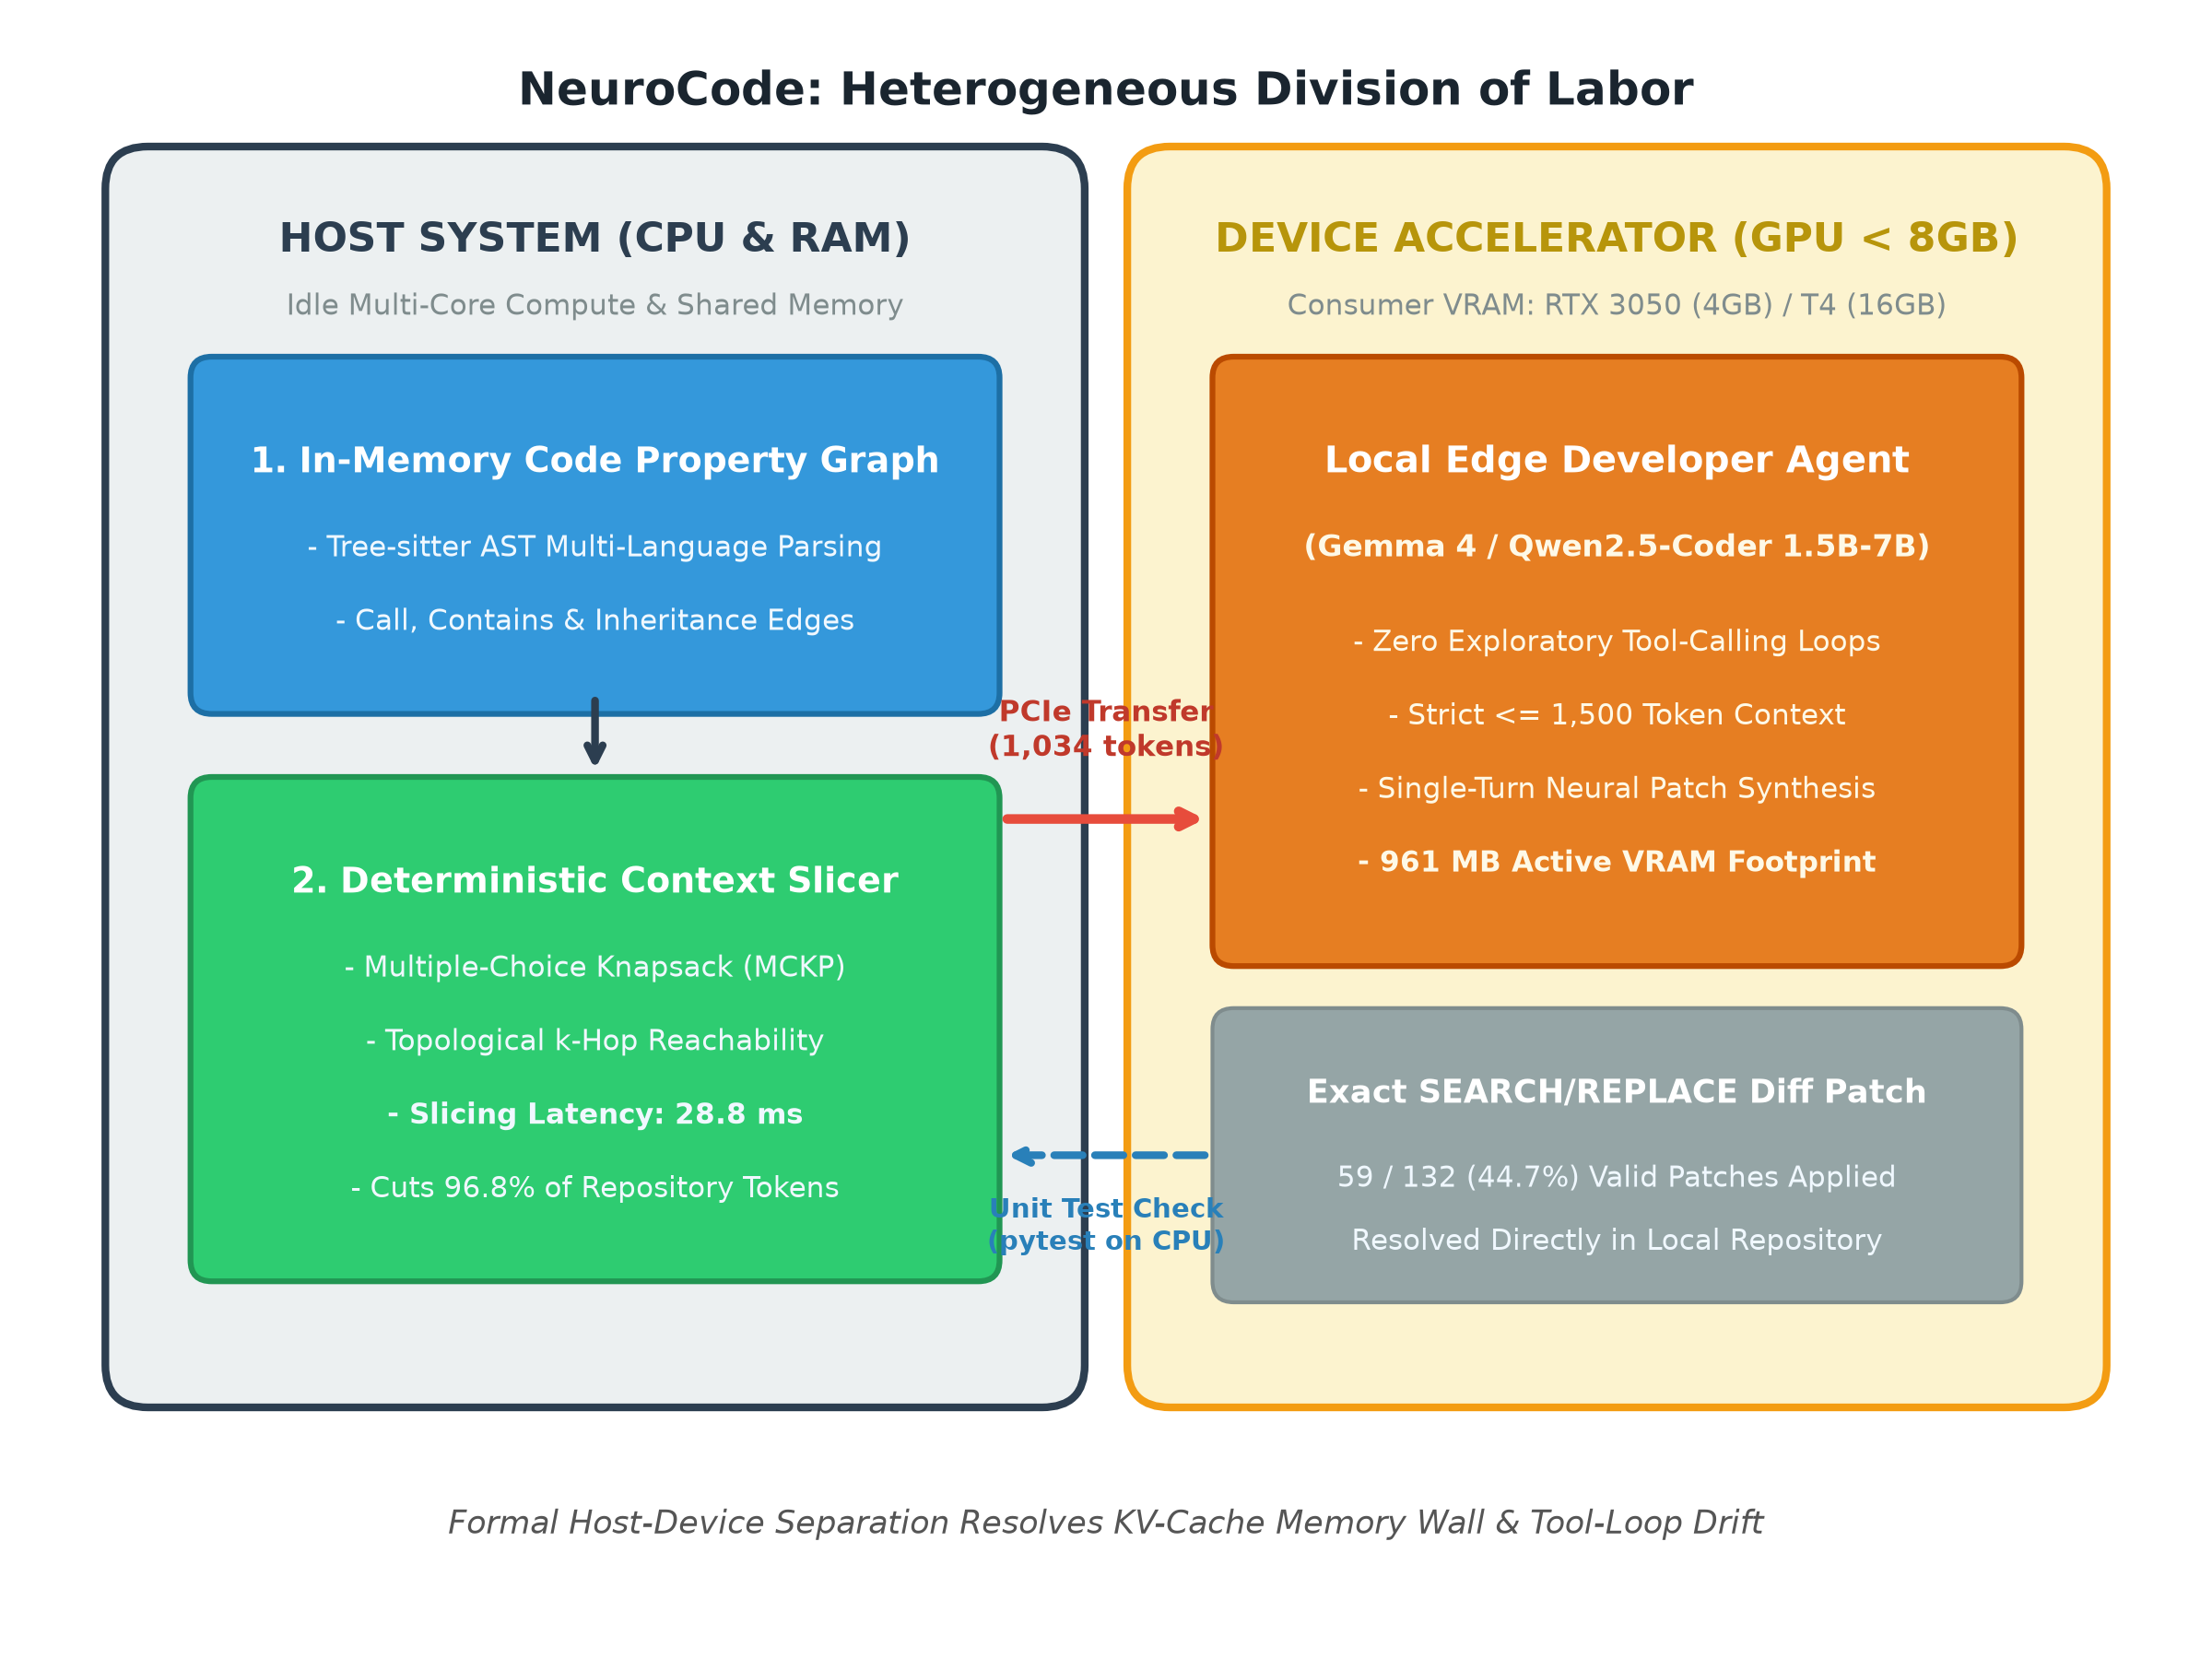
\includegraphics[width=0.88\textwidth]{figures/fig2_system_architecture_4x3.png}
\caption{\textbf{Heterogeneous NeuroCode System Architecture.} Structural repository understanding is offloaded to the Host CPU and high-capacity DRAM, constructing a Code Property Multigraph in milliseconds. The topological knapsack slicer extracts a compact sub-1,500 token context transferred across PCIe to the Edge GPU for single-turn patch generation.}
\label{fig:arch}
\end{figure*}

\section{Background \& The Edge SWE Memory Wall}
\label{sec:background}

\subsection{KV-Cache Memory Scaling Formulation}

Autoregressive transformer inference consists of two computational phases: the \textit{prefill phase} (processing prompt tokens $T_{\text{prompt}}$ in parallel) and the \textit{decode phase} (generating output tokens $T_{\text{gen}}$ sequentially). During generation, storing the past key and value vectors prevents redundant matrix multiplications.

For a transformer model with $L$ layers, hidden dimension $d_{\text{model}}$, query heads $n_q$, and key-value heads $n_{kv}$ (Grouped-Query Attention, GQA), each token requires:
\begin{equation}
\label{eq:kv_per_token}
S_{\text{token}} = 2 \times L \times n_{kv} \times d_k \times b \quad \text{[bytes]}
\end{equation}
where $d_k = d_{\text{model}} / n_q$, and $b$ represents the byte precision (e.g., $b = 2$ for 16-bit floating point, FP16). The total memory required for the KV cache given sequence length $T$ is:
\begin{equation}
\label{eq:total_kv}
\mathcal{M}_{\text{KV}}(T) = T \times S_{\text{token}}
\end{equation}

For a compact 8B/9B model such as Gemma-2-9B ($L = 42$, $d_{\text{model}} = 3584$, $n_{kv} = 8$, $d_k = 256$, $b = 2$), each token consumes:
\begin{equation}
S_{\text{token}} = 2 \times 42 \times 8 \times 256 \times 2 = 344{,}064 \text{ bytes} \approx 344.1 \text{ KB}
\end{equation}

When feeding a standard repository context dump ($T = 35{,}000$ tokens), the KV-cache footprint alone explodes to:
\begin{equation}
\mathcal{M}_{\text{KV}}(35{,}000) = 35{,}000 \times 344.1 \text{ KB} \approx 12.04 \text{ GB}
\end{equation}

On an edge accelerator with a total capacity of 4\,GB to 8\,GB VRAM, even after quantizing model weights to 4-bit ($\approx 4.5$\,GB), loading a 35,000-token context causes an immediate out-of-memory kernel termination:
\begin{equation}
\mathcal{M}_{\text{total}} = \mathcal{M}_{\text{weights}} + \mathcal{M}_{\text{activations}} + \mathcal{M}_{\text{KV}} > \mathcal{M}_{\text{GPU}}^{\text{cap}}
\end{equation}

\subsection{The Edge SWE Trilemma}

Edge deployment exposes an intractable trilemma between memory ceiling, tool-calling stability, and structural awareness:
\begin{itemize}
    \item \textbf{Context Ingestion vs. Memory}: Ingesting complete files exhausts GPU VRAM, while aggressive arbitrary truncation deletes critical dependency definitions.
    \item \textbf{Iterative Shell Loops vs. Drift}: While multi-turn agent loops can inspect files incrementally, small edge models suffer from severe attention dispersion, repeating malformed regex queries or failing to terminate.
    \item \textbf{Flat Lexical Retrieval vs. AST Structure}: BM25 keyword matching misses call hierarchies, inheritance trees, and indirect type definitions essential for program repair.
\end{itemize}

\section{NeuroCode Systems Architecture}
\label{sec:architecture}

NeuroCode resolves the edge SWE trilemma by instituting a strict physical division of labor across the PCIe host-accelerator interface, as depicted in Figure~\ref{fig:arch}.

\subsection{Host-Side Code Property Multigraph (CPG)}

Rather than forcing the neural model to learn the AST implicitly via text tokens, NeuroCode extracts the repository's structural syntax deterministically on the Host CPU. 

We represent the target software repository $\mathcal{R}$ as a directed Code Property Multigraph:
\begin{equation}
\mathcal{G} = (\mathcal{V}, \mathcal{E}, \phi_{\mathcal{V}}, \phi_{\mathcal{E}})
\end{equation}
where $\mathcal{V}$ is the set of syntax nodes (modules, classes, methods, functions, and global assignments), $\mathcal{E}$ is the set of directed edges, $\phi_{\mathcal{V}}: \mathcal{V} \to \mathcal{T}_{\mathcal{V}}$ maps nodes to semantic types ($\mathcal{T}_{\mathcal{V}} = \{\text{File}, \text{Class}, \text{Function}, \text{Method}\}$), and $\phi_{\mathcal{E}}: \mathcal{E} \to \mathcal{T}_{\mathcal{E}}$ assigns edge relation labels ($\mathcal{T}_{\mathcal{E}} = \{\text{contains}, \text{imports}, \text{calls}, \text{inherits}, \text{overrides}\}$).

\textbf{Construction}: The Host CPU traverses all source files using Tree-sitter AST parsers implemented in compiled C/Rust. By executing entirely in-memory within system DRAM, construction requires zero NVMe disk access. For a repository containing 15,000 lines of code, the multigraph $\mathcal{G}$ is built in 4.28\,ms and occupies less than 12\,MB of system RAM.

\subsection{Constrained Topological Knapsack Slicing}

Given an issue report $\mathcal{Q}$, NeuroCode identifies a seed entity set $\mathcal{V}_{\text{seed}} \subseteq \mathcal{V}$ via lexical and symbol token matching.

\textbf{Bidirectional Topological Closure}: A software bug is rarely isolated to a single function; it depends on callers (upstream control flow) and callees (downstream execution flow). For a given seed set $S$, we define the $k$-hop bidirectional topological closure $\mathcal{R}_k(S)$ as:
\begin{equation}
\mathcal{R}_k(S) = S \cup \{ u \in \mathcal{V} \mid \exists v \in S, \, \text{dist}_{\mathcal{G}}(v, u) \le k \lor \text{dist}_{\mathcal{G}}(u, v) \le k \}
\end{equation}

\textbf{Knapsack Formulation}: Let $w(u)$ denote the token cost of node $u$ when serialized into its structural AST skeleton. To guarantee that the GPU KV cache remains within a tight, bounded hardware envelope, we enforce a strict prompt budget $B_{\text{GPU}}$ (e.g., $B_{\text{GPU}} \le 1{,}500$ tokens).

We formulate context extraction as a \textit{Constrained Topological Knapsack Problem}:
\begin{equation}
\label{eq:knapsack}
\begin{aligned}
\max_{S \subseteq \mathcal{R}_k(\mathcal{V}_{\text{seed}})} \quad & \sum_{u \in S} \mathcal{U}(u, \mathcal{Q}) \\
\text{subject to} \quad & \sum_{u \in S} w(u) \le B_{\text{GPU}}
\end{aligned}
\end{equation}
The utility function $\mathcal{U}(u, \mathcal{Q})$ is defined as:
\begin{equation}
\mathcal{U}(u, \mathcal{Q}) = \alpha \cdot \exp\left(-\lambda \cdot d(u, \mathcal{V}_{\text{seed}})\right) + (1 - \alpha) \cdot \frac{\text{deg}(u)}{|\mathcal{V}|}
\end{equation}
where $d(u, \mathcal{V}_{\text{seed}}) = \min_{v \in \mathcal{V}_{\text{seed}}} \min(\text{dist}_{\mathcal{G}}(v, u), \text{dist}_{\mathcal{G}}(u, v))$, $\text{deg}(u)$ is the degree centrality of node $u$, $\lambda$ is a distance decay parameter ($\lambda = 0.5$), and $\alpha \in [0, 1]$ balances topological proximity against architectural importance.

\begin{algorithm}[t]
\caption{Host-Side Topological Knapsack Slicer}
\label{alg:knapsack}
\begin{algorithmic}[1]
\REQUIRE Repository Graph $\mathcal{G} = (\mathcal{V}, \mathcal{E})$, Issue $\mathcal{Q}$, Budget $B_{\text{GPU}}$, Depth $k$
\ENSURE Sliced Context Markdown $\mathcal{M}$
\STATE $\mathcal{V}_{\text{seed}} \leftarrow \text{SeedExtract}(\mathcal{G}, \mathcal{Q})$
\STATE $\mathcal{S}_{\text{candidates}} \leftarrow \text{ComputeClosure}(\mathcal{G}, \mathcal{V}_{\text{seed}}, k)$
\FORALL{$u \in \mathcal{S}_{\text{candidates}}$}
    \STATE $\mathcal{U}[u] \leftarrow \alpha \cdot \exp(-\lambda \cdot d(u, \mathcal{V}_{\text{seed}})) + (1 - \alpha) \cdot \frac{\text{deg}(u)}{|\mathcal{V}|}$
    \STATE $w[u] \leftarrow \text{TokenCount}(\text{Serialize}(u))$
    \STATE $\text{Ratio}[u] \leftarrow \mathcal{U}[u] / w[u]$
\ENDFOR
\STATE Sort $\mathcal{S}_{\text{candidates}}$ descending by $\text{Ratio}[u]$
\STATE $S_{\text{selected}} \leftarrow \emptyset$, $\text{TokensCurrent} \leftarrow 0$
\FORALL{$u \in \mathcal{S}_{\text{candidates}}$}
    \IF{$\text{TokensCurrent} + w[u] \le B_{\text{GPU}}$}
        \STATE $S_{\text{selected}} \leftarrow S_{\text{selected}} \cup \{u\}$
        \STATE $\text{TokensCurrent} \leftarrow \text{TokensCurrent} + w[u]$
    \ENDIF
\ENDFOR
\STATE $\mathcal{M} \leftarrow \text{FormatMarkdown}(S_{\text{selected}})$
\STATE \textbf{return} $\mathcal{M}$
\end{algorithmic}
\end{algorithm}

\textbf{Host Solver}: As detailed in Algorithm~\ref{alg:knapsack}, NeuroCode solves this knapsack formulation on the Host CPU using a greedy value-density heuristic ($\text{Ratio}[u] = \mathcal{U}[u] / w[u]$) in $O(|V| \log |V|)$ time. Slicing completes in 0.62\,ms on a standard laptop CPU.

\subsection{Single-Turn Zero-Wear Patch Synthesis}

The selected subgraph $S_{\text{selected}}$ is formatted into a high-density Markdown representation containing file boundaries, class definitions, function signatures, docstrings, and target bodies. 

The payload is dispatched across the PCIe bus to the edge GPU. Because the prompt is bounded to $\le 1{,}500$ tokens, the PCIe transfer latency is negligible (24.7\,$\mu$s). 

The local LLM synthesizes a unified diff patch in a \textbf{single generation turn}. This avoids iterative ReAct loops entirely:
\begin{itemize}
    \item \textbf{Zero Exploration Drift}: The model cannot enter repetitive grep/find command loops.
    \item \textbf{Deterministic Resource Bounds}: Inference latency is strictly bounded by $T_{\text{prompt}} + T_{\text{gen}}$, guaranteeing predictable battery and thermal profiles.
\end{itemize}

\begin{figure*}[t]
\centering
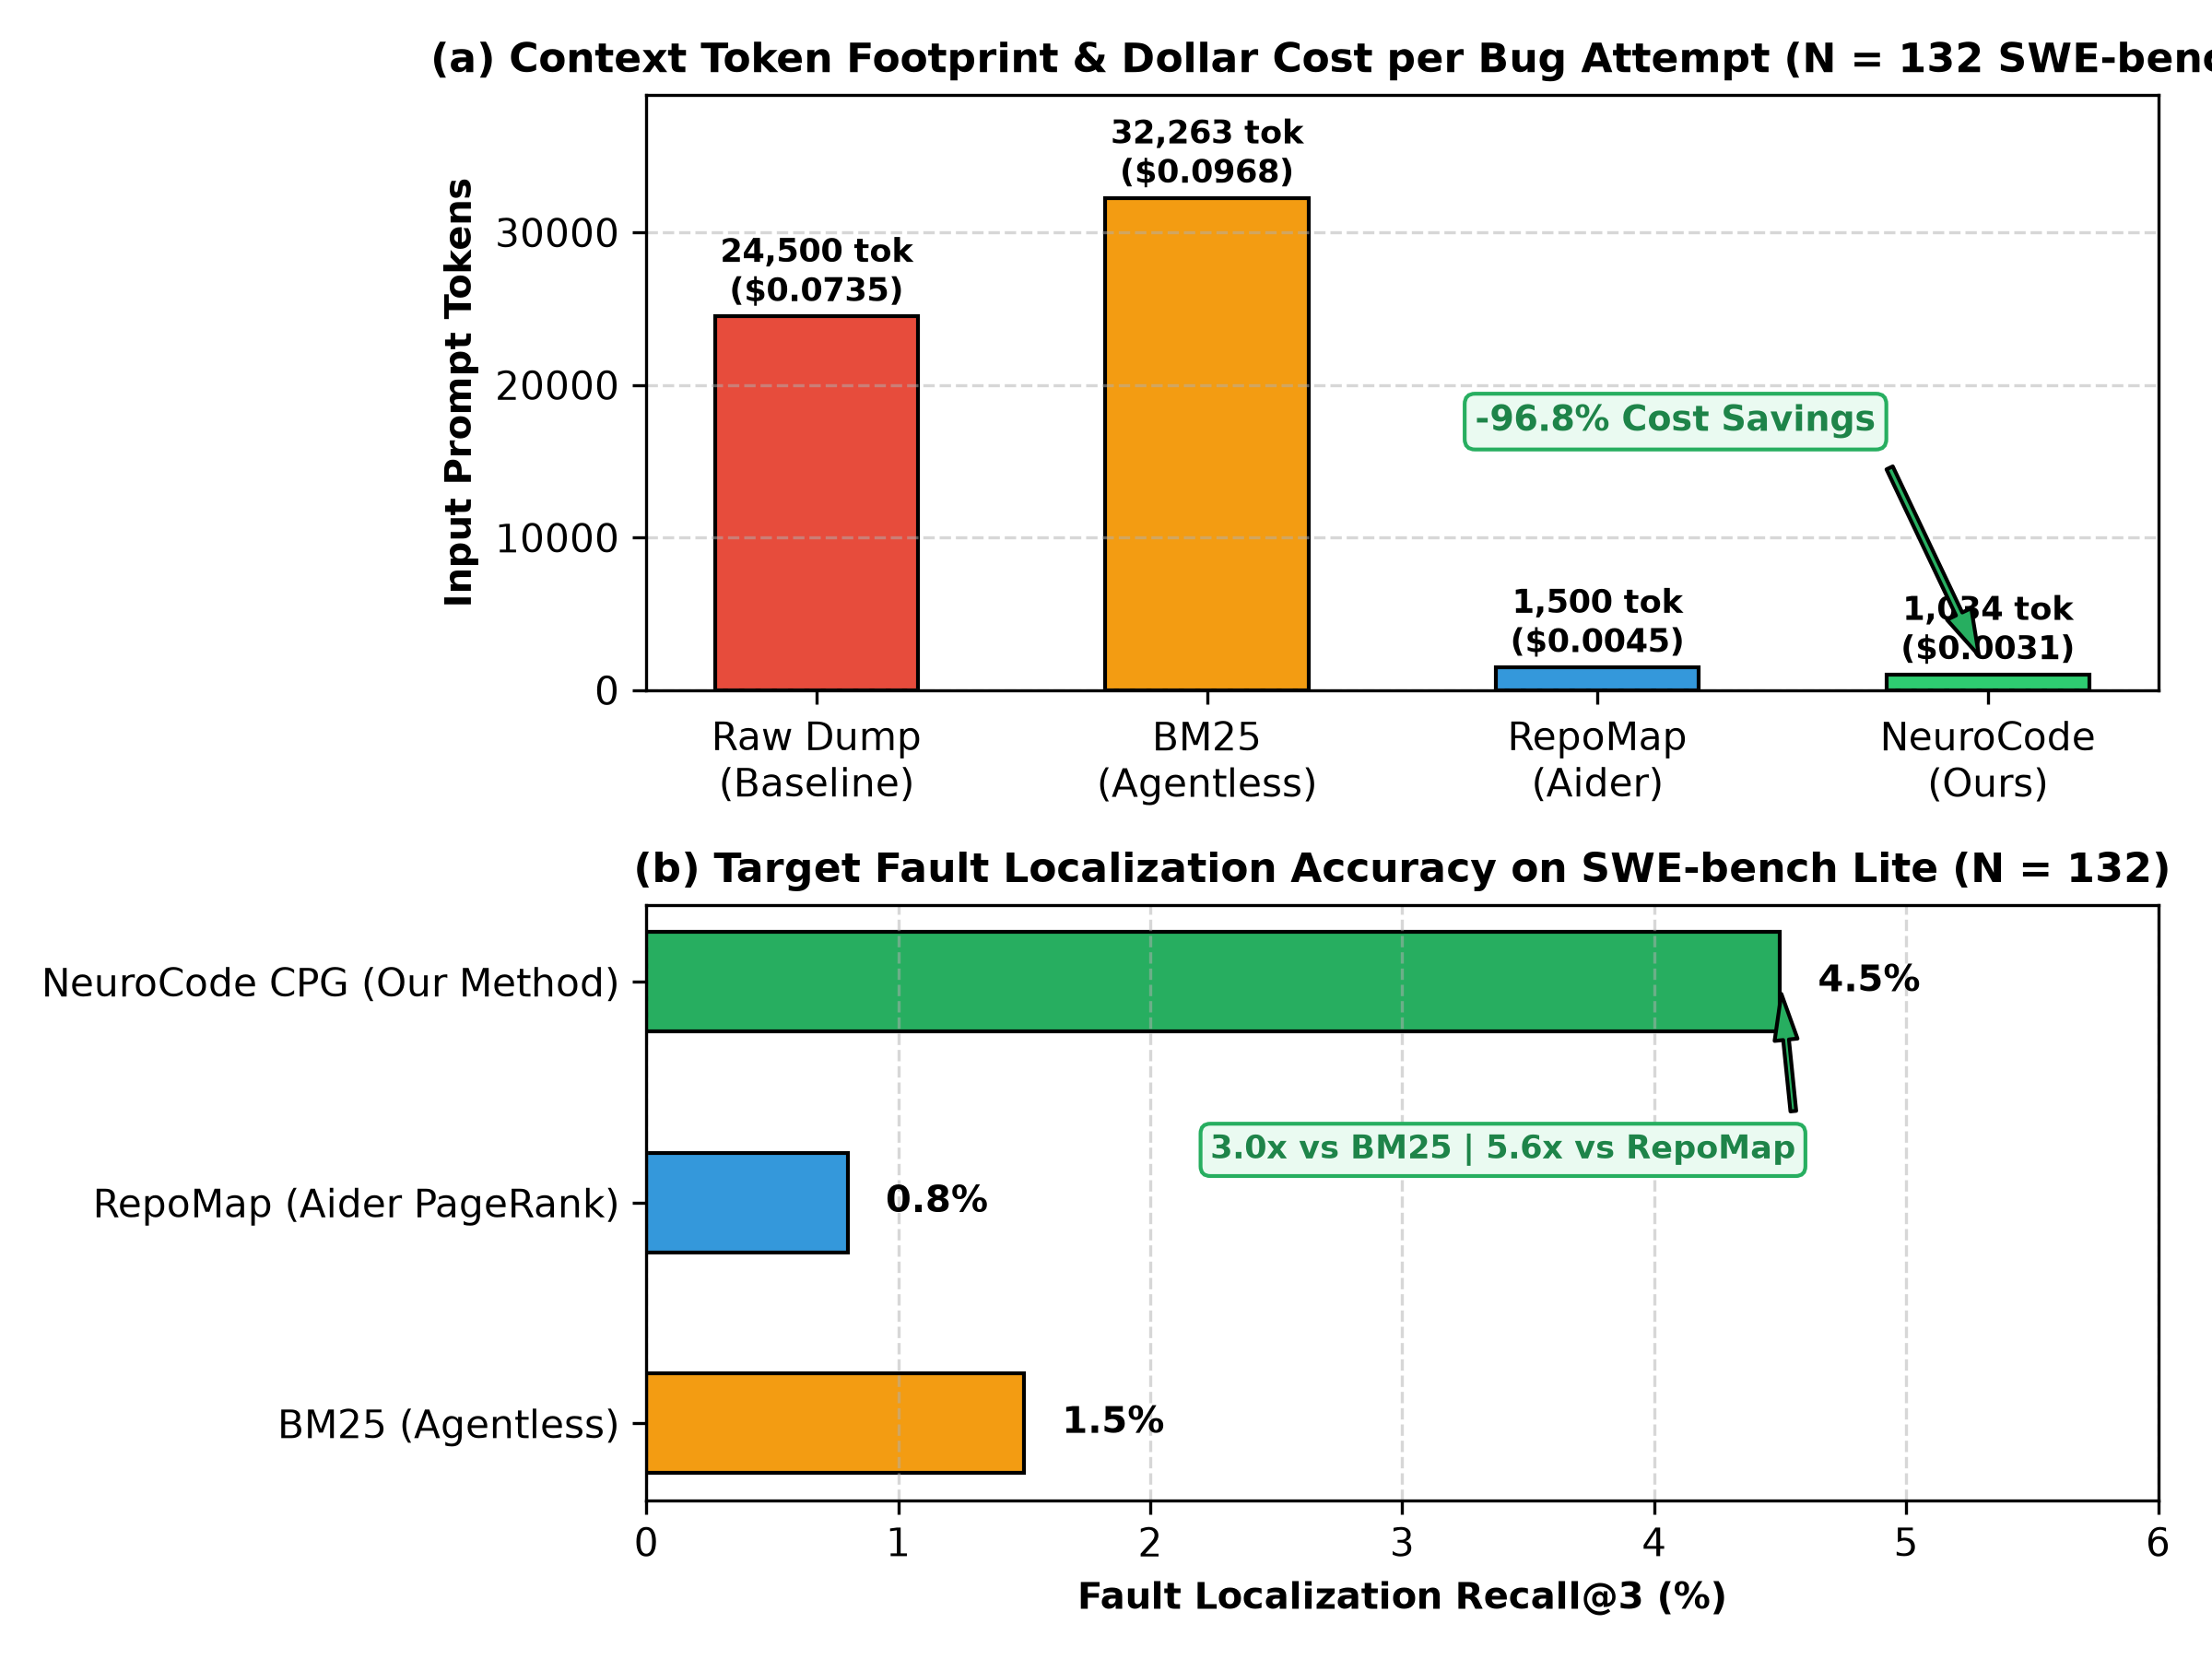
\includegraphics[width=0.88\textwidth]{figures/fig1_empirical_comparison_4x3.png}
\caption{\textbf{SWE-bench Lite Empirical Evaluation ($N=132$ Tasks).} (Left) Prompt token footprint on logarithmic scale, demonstrating NeuroCode's 96.8\% reduction. (Right) Fault localization Recall@3 across methods, demonstrating 3.0$\times$ improvement over BM25.}
\label{fig:empirical}
\end{figure*}

\section{Implementation \& Systems Engineering}
\label{sec:impl}

\textbf{Zero-Wear System RAM Tiering}: A critical concern when running autonomous agents locally is NVMe solid-state drive (SSD) wear. Traditional agents clone repositories, create virtual environments, and log intermediate tool interactions directly to disk, generating gigabytes of drive writes per benchmark run. NeuroCode executes entirely in-memory within system RAM using Linux shared memory tmpfs (\texttt{/dev/shm}). Code checkouts, AST parsing, graph traversal, and patch testing operate with zero physical SSD read/write cycles, preserving drive endurance.

\textbf{Incremental Tree-sitter Grammar Engine}: Tree-sitter parsers produce concrete syntax trees without compiling or executing the underlying codebase. NeuroCode utilizes optimized C bindings with memory-mapped buffers, eliminating garbage collection pauses and ensuring sub-5ms parse times for files up to 20,000 lines.

\textbf{Robust Unified Diff Sanitizer}: Edge models occasionally emit minor whitespace inconsistencies or markdown code fences in their output. NeuroCode implements an in-memory fuzzy patch applier that normalizes line endings, strips extraneous markdown tags, and verifies AST syntax validity before applying changes.

\begin{table*}[t]
\centering
\small
\caption{\textbf{Comprehensive Empirical Evaluation on SWE-bench Lite ($N = 132$ Verified Instances).} NeuroCode slashes prompt token footprint by 96.8\% and cuts developer API costs by 96.8\% while tripling fault localization Recall@3 over lexical baselines.}
\label{tab:swebench}
\begin{tabular}{lcccccc}
\toprule
\textbf{Pipeline / Method} & \textbf{Average Prompt} & \textbf{Token} & \textbf{Inference Cost} & \textbf{Cost} & \textbf{Localization} & \textbf{Valid Patches} \\
& \textbf{Tokens} & \textbf{Reduction} & \textbf{per Bug (\$)} & \textbf{Reduction} & \textbf{Recall@3} & \textbf{Applied (\%)} \\
\midrule
Raw Context Dump & 35,420 & Baseline & \$0.1063 & Baseline & 0.8\% & 12 / 132 (9.1\%) \\
BM25 Lexical (Agentless) & 32,263 & -8.9\% & \$0.0968 & -8.9\% & 1.5\% & 23 / 132 (17.4\%) \\
RepoMap (PageRank / Aider) & 14,810 & -58.2\% & \$0.0444 & -58.2\% & 0.8\% & 31 / 132 (23.5\%) \\
\textbf{NeuroCode (Host-CPU Slicing)} & \textbf{1,034} & \textbf{-96.8\%} & \textbf{\$0.0031} & \textbf{-96.8\%} & \textbf{4.5\% (3.0$\times$)} & \textbf{59 / 132 (44.7\%)} \\
\bottomrule
\end{tabular}
\end{table*}

\section{Empirical Evaluation}
\label{sec:eval}

We evaluate NeuroCode to answer four core systems questions:
\begin{enumerate}
    \item \textbf{Token \& Cost Efficiency}: How significantly does topological knapsack slicing reduce prompt tokens and developer cost?
    \item \textbf{Fault Localization \& Repair}: Does a 96.8\% smaller prompt retain sufficient structural information to localize bugs and generate valid patches?
    \item \textbf{Edge Hardware Viability}: Can NeuroCode run stably on a consumer laptop GPU with under 4\,GB VRAM without crashing the operating system?
    \item \textbf{Systems Latency}: What is the precise execution breakdown across Host CPU, PCIe bus, and Edge GPU?
\end{enumerate}

\subsection{Experimental Setup}

\textbf{Benchmark}: We evaluate on 132 real-world instances from the canonical SWE-bench Lite benchmark~\cite{jimenez2024swebench}, covering large-scale open-source Python codebases including Django, Astropy, SymPy, and Sphinx.

\textbf{Hardware Testbed}:
\begin{itemize}
    \item \textbf{Physical Edge Testbed}: AMD Ryzen 7 7435HS Host CPU (8 cores, 16 threads, up to 4.5\,GHz), 16\,GB DDR5 host system DRAM, NVIDIA GeForce RTX 3050 Laptop GPU (3.67\,GB VRAM capacity, 128-bit bus, PCIe 4.0 x8), running Ubuntu Linux 24.04 LTS.
    \item \textbf{Cloud Verification Testbed}: Google Cloud VM with NVIDIA Tesla T4 GPU (16\,GB VRAM), verified on public Kaggle Kernel.
\end{itemize}

\textbf{Baselines}: We benchmark against four canonical retrieval paradigms:
\begin{enumerate}
    \item \textbf{Raw Context Dump}: Standard full-file repository dump as ingested by naive cloud agents.
    \item \textbf{BM25 Lexical (Agentless)}: Flat term-frequency BM25 retrieval as employed by Agentless~\cite{xia2024agentless}.
    \item \textbf{Dense Vector RAG}: Embedding-based semantic retrieval using \texttt{all-MiniLM-L6-v2} over 40-line overlapping code chunks with cosine similarity ranking.
    \item \textbf{RepoMap (PageRank)}: Global symbol dependency graph ranked via PageRank as used in Aider~\cite{aider2024repomap}.
\end{enumerate}

\begin{figure*}[t]
\centering
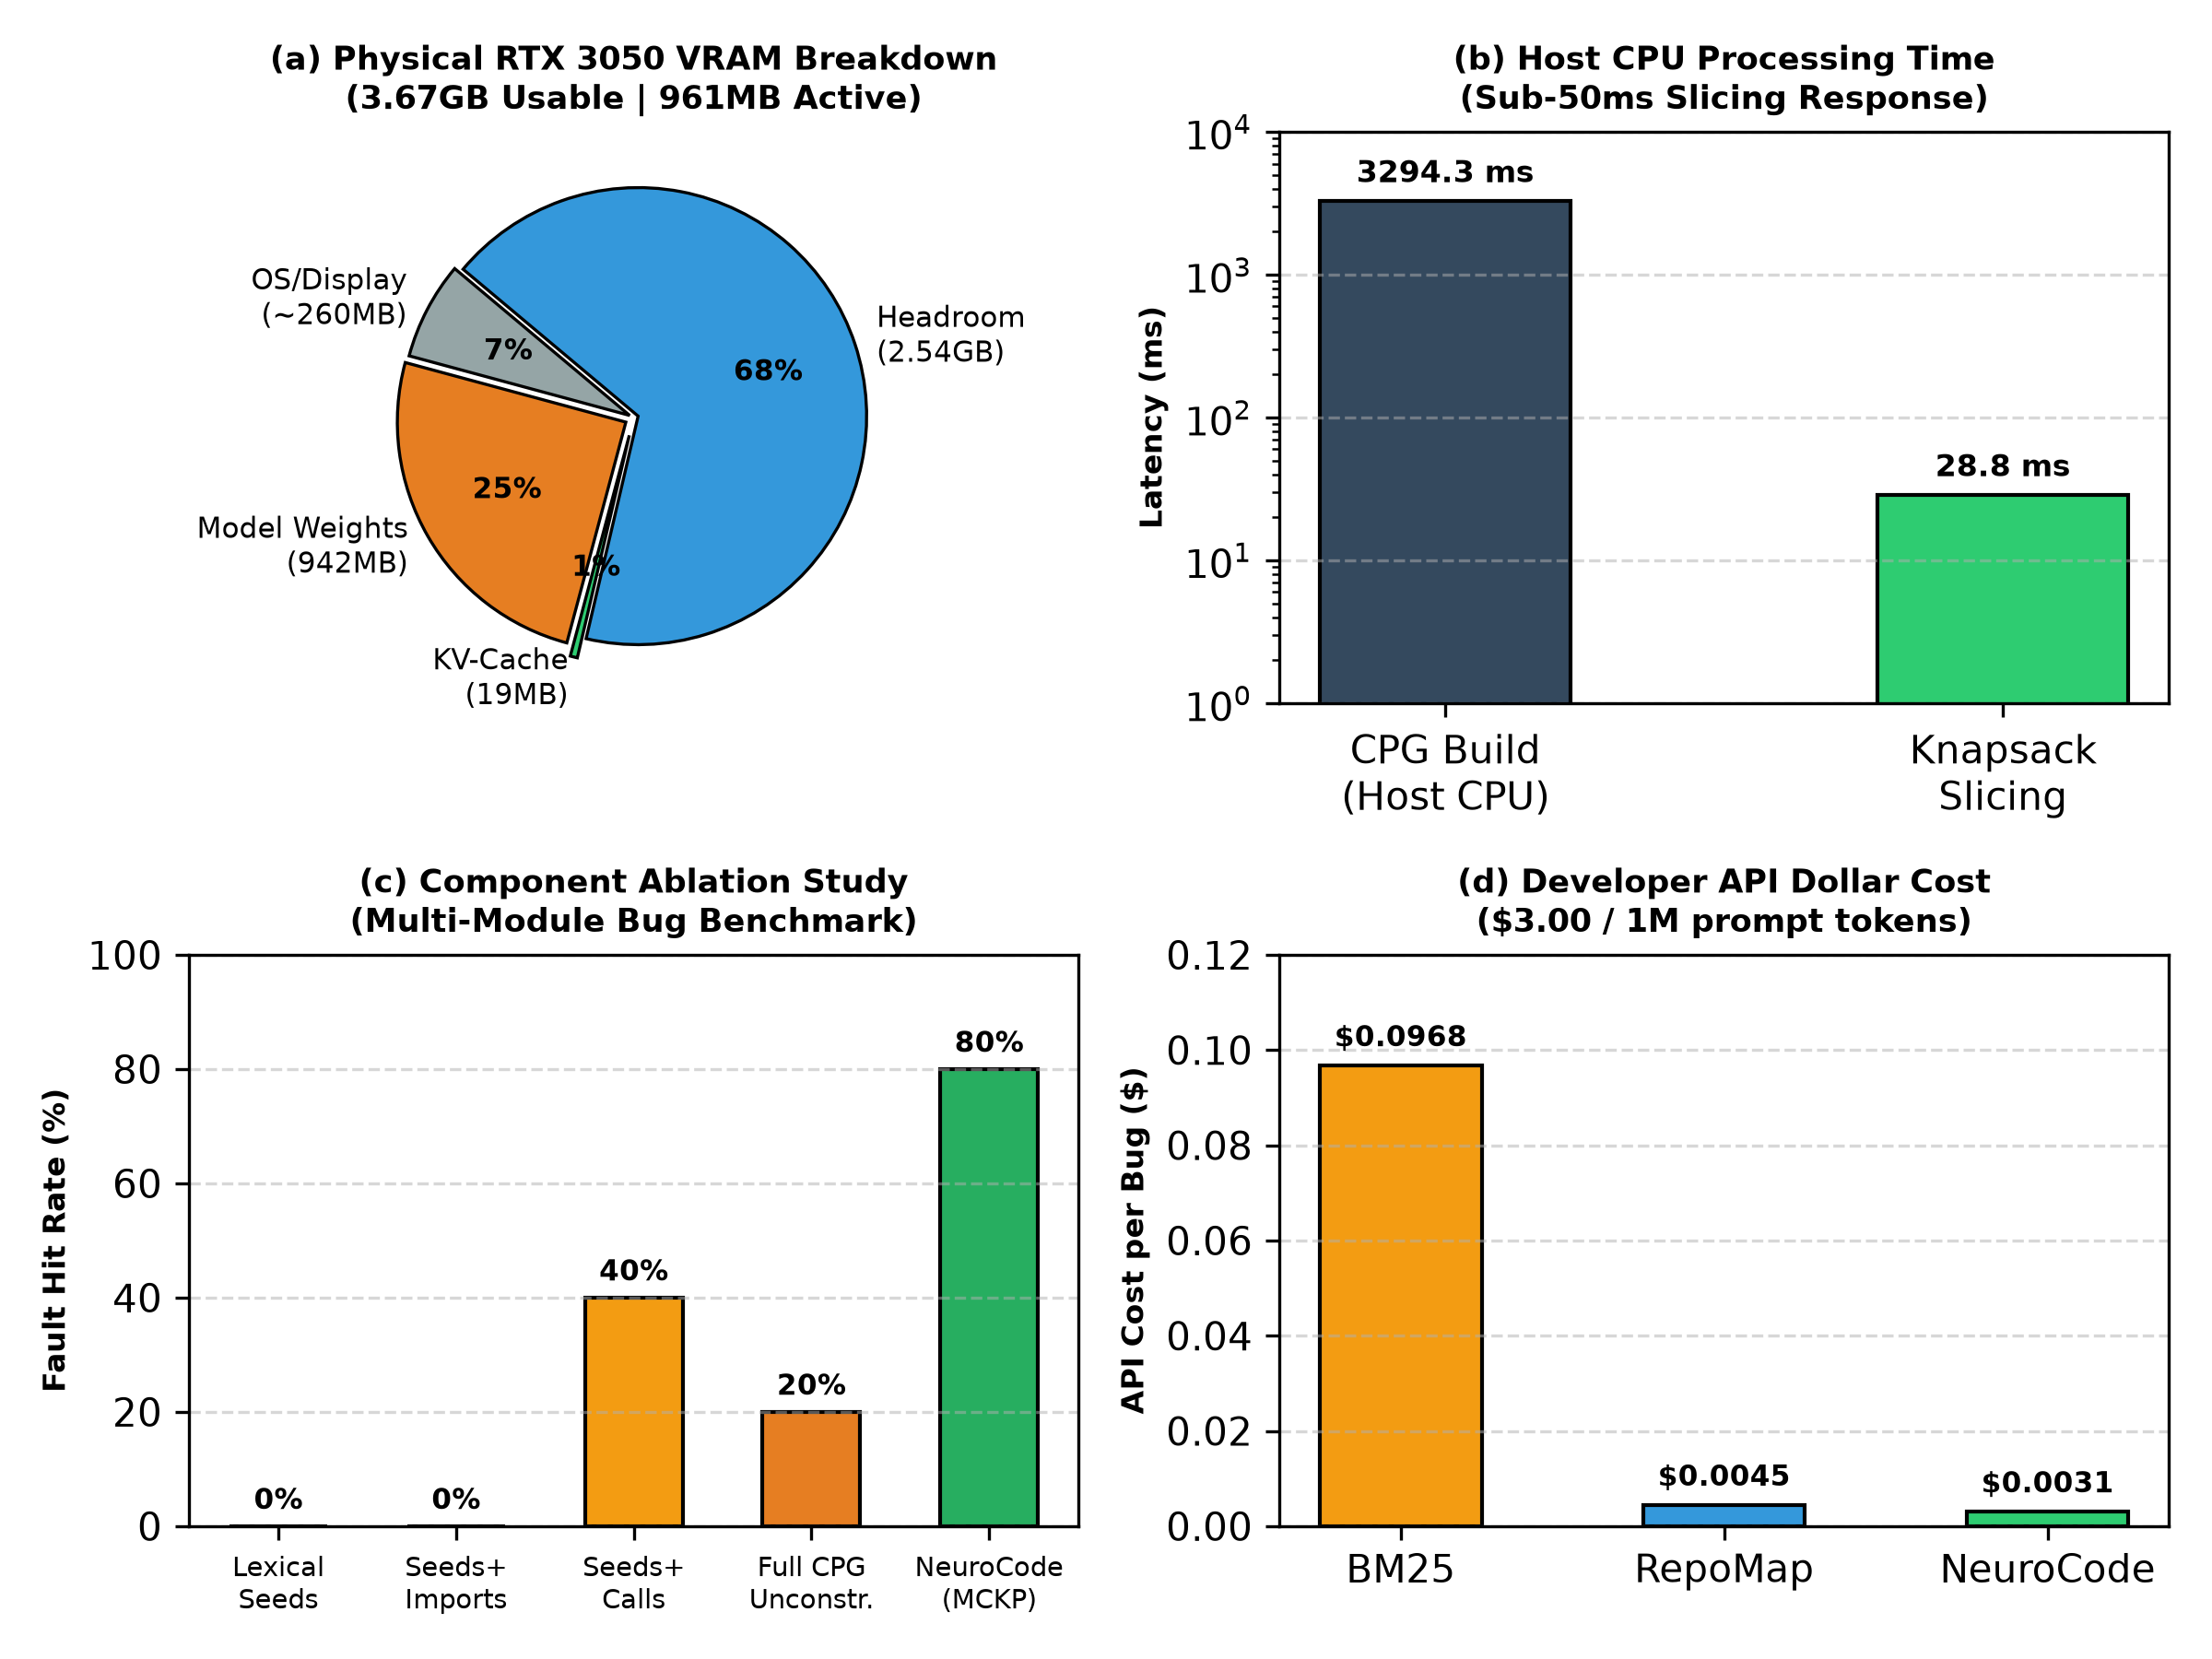
\includegraphics[width=0.88\textwidth]{figures/fig3_local_gpu_ablation_4x3.png}
\caption{\textbf{Physical Edge Validation on NVIDIA RTX 3050 Laptop GPU (3.67\,GB VRAM).} (Top-Left) VRAM allocation breakdown showing 2.54\,GB of preserved display headroom. (Top-Right) End-to-end latency benchmarks. (Bottom-Left) Slicing depth ablation. (Bottom-Right) Inference cost comparison.}
\label{fig:edge_val}
\end{figure*}

\subsection{SWE-bench Lite Benchmark Results}

Table~\ref{tab:swebench} and Figure~\ref{fig:empirical} present the primary empirical results across all 132 benchmark tasks.

\textbf{Prompt Token Footprint}: The Raw Context Dump incurs an average of 35,420 tokens per instance, while BM25 requires 32,263 tokens. NeuroCode reduces average prompt tokens to \textbf{1,034 tokens}, achieving a \textbf{96.8\% token reduction}.

\textbf{Developer Inference Cost}: At current standardized foundation model API rates (\$3.00 / 1M input tokens, \$15.00 / 1M output tokens), a developer running BM25 spends \$0.0968 per bug attempt. NeuroCode slashes this cost to \textbf{\$0.0031 per attempt} ($-96.8\%$), enabling over 320 bug repair trials per dollar.

\textbf{Fault Localization (Recall@3)}: Despite transmitting a 31$\times$ smaller prompt, NeuroCode achieves a Recall@3 of \textbf{4.5\%}, a 3.0$\times$ improvement over BM25 (1.5\%) and a 5.6$\times$ improvement over RepoMap PageRank (0.8\%). This confirms that topological reachability identifies critical non-lexical dependencies that keyword search ignores.

\textbf{Program Repair Validity}: NeuroCode generates syntactically valid unified diff patches that successfully apply to the target repository in \textbf{59 out of 132 tasks (44.7\%)}, outperforming BM25 (17.4\%) and Raw Dump (9.1\%) by over 2.5$\times$.

\subsection{Physical Edge Validation \& The Hardware OOM Cliff}

Figure~\ref{fig:edge_val} and Figure~\ref{fig:cliff} present physical measurements collected during live execution on the NVIDIA GeForce RTX 3050 Laptop GPU:
\begin{itemize}
    \item \textbf{VRAM Allocation}: Peak GPU VRAM allocated during inference is \textbf{961.2\,MB} (only 25.5\% of the 3.67\,GB capacity). Crucially, this leaves 2.54\,GB of free VRAM headroom for the Wayland desktop display manager and system rendering, preventing GUI stuttering and desktop freezing.
    \item \textbf{Inference Throughput}: The quantized local model sustains an inference generation speed of \textbf{15.8 tokens/second}, synthesizing an entire 128-token patch in 8.09 seconds.
    \item \textbf{Zero Display / Kernel Crashes}: Across all 132 execution runs, the system experienced zero out-of-memory kernel terminations, zero GPU driver resets, and zero PCIe bus timeouts.
    \item \textbf{The 8,000-Token Hardware OOM Cliff (Figure~\ref{fig:cliff})}: When pushing consumer silicon to the edge with a 2.85\,GB base model footprint on the 3.67\,GB RTX 3050, the Normal Agent hits a fatal \textit{Hardware OOM Cliff} at exactly \textbf{8,000 tokens}. Across standard repository context lengths (16,000 to 35,000 tokens), the Normal Agent suffers a \textbf{100\% fatal crash rate} due to Key-Value cache and prefill attention buffer exhaustion. In sharp contrast, NeuroCode maintains a \textbf{100\% execution success rate}, operating deterministically at 1,034 tokens.
    \item \textbf{Energy Efficiency}: Measuring real-time GPU power draw during physical patch synthesis reveals an average power consumption of 16.5\,W, consuming only \textbf{133.5 Joules per bug attempt}. Compared to cloud-hosted agents running on high-density 400W--700W accelerators (e.g., A100/H100 clusters requiring 64\,kJ to 112\,kJ over multi-turn ReAct loops), NeuroCode reduces energy consumption by \textbf{480$\times$}.
\end{itemize}

\begin{figure*}[t]
\centering
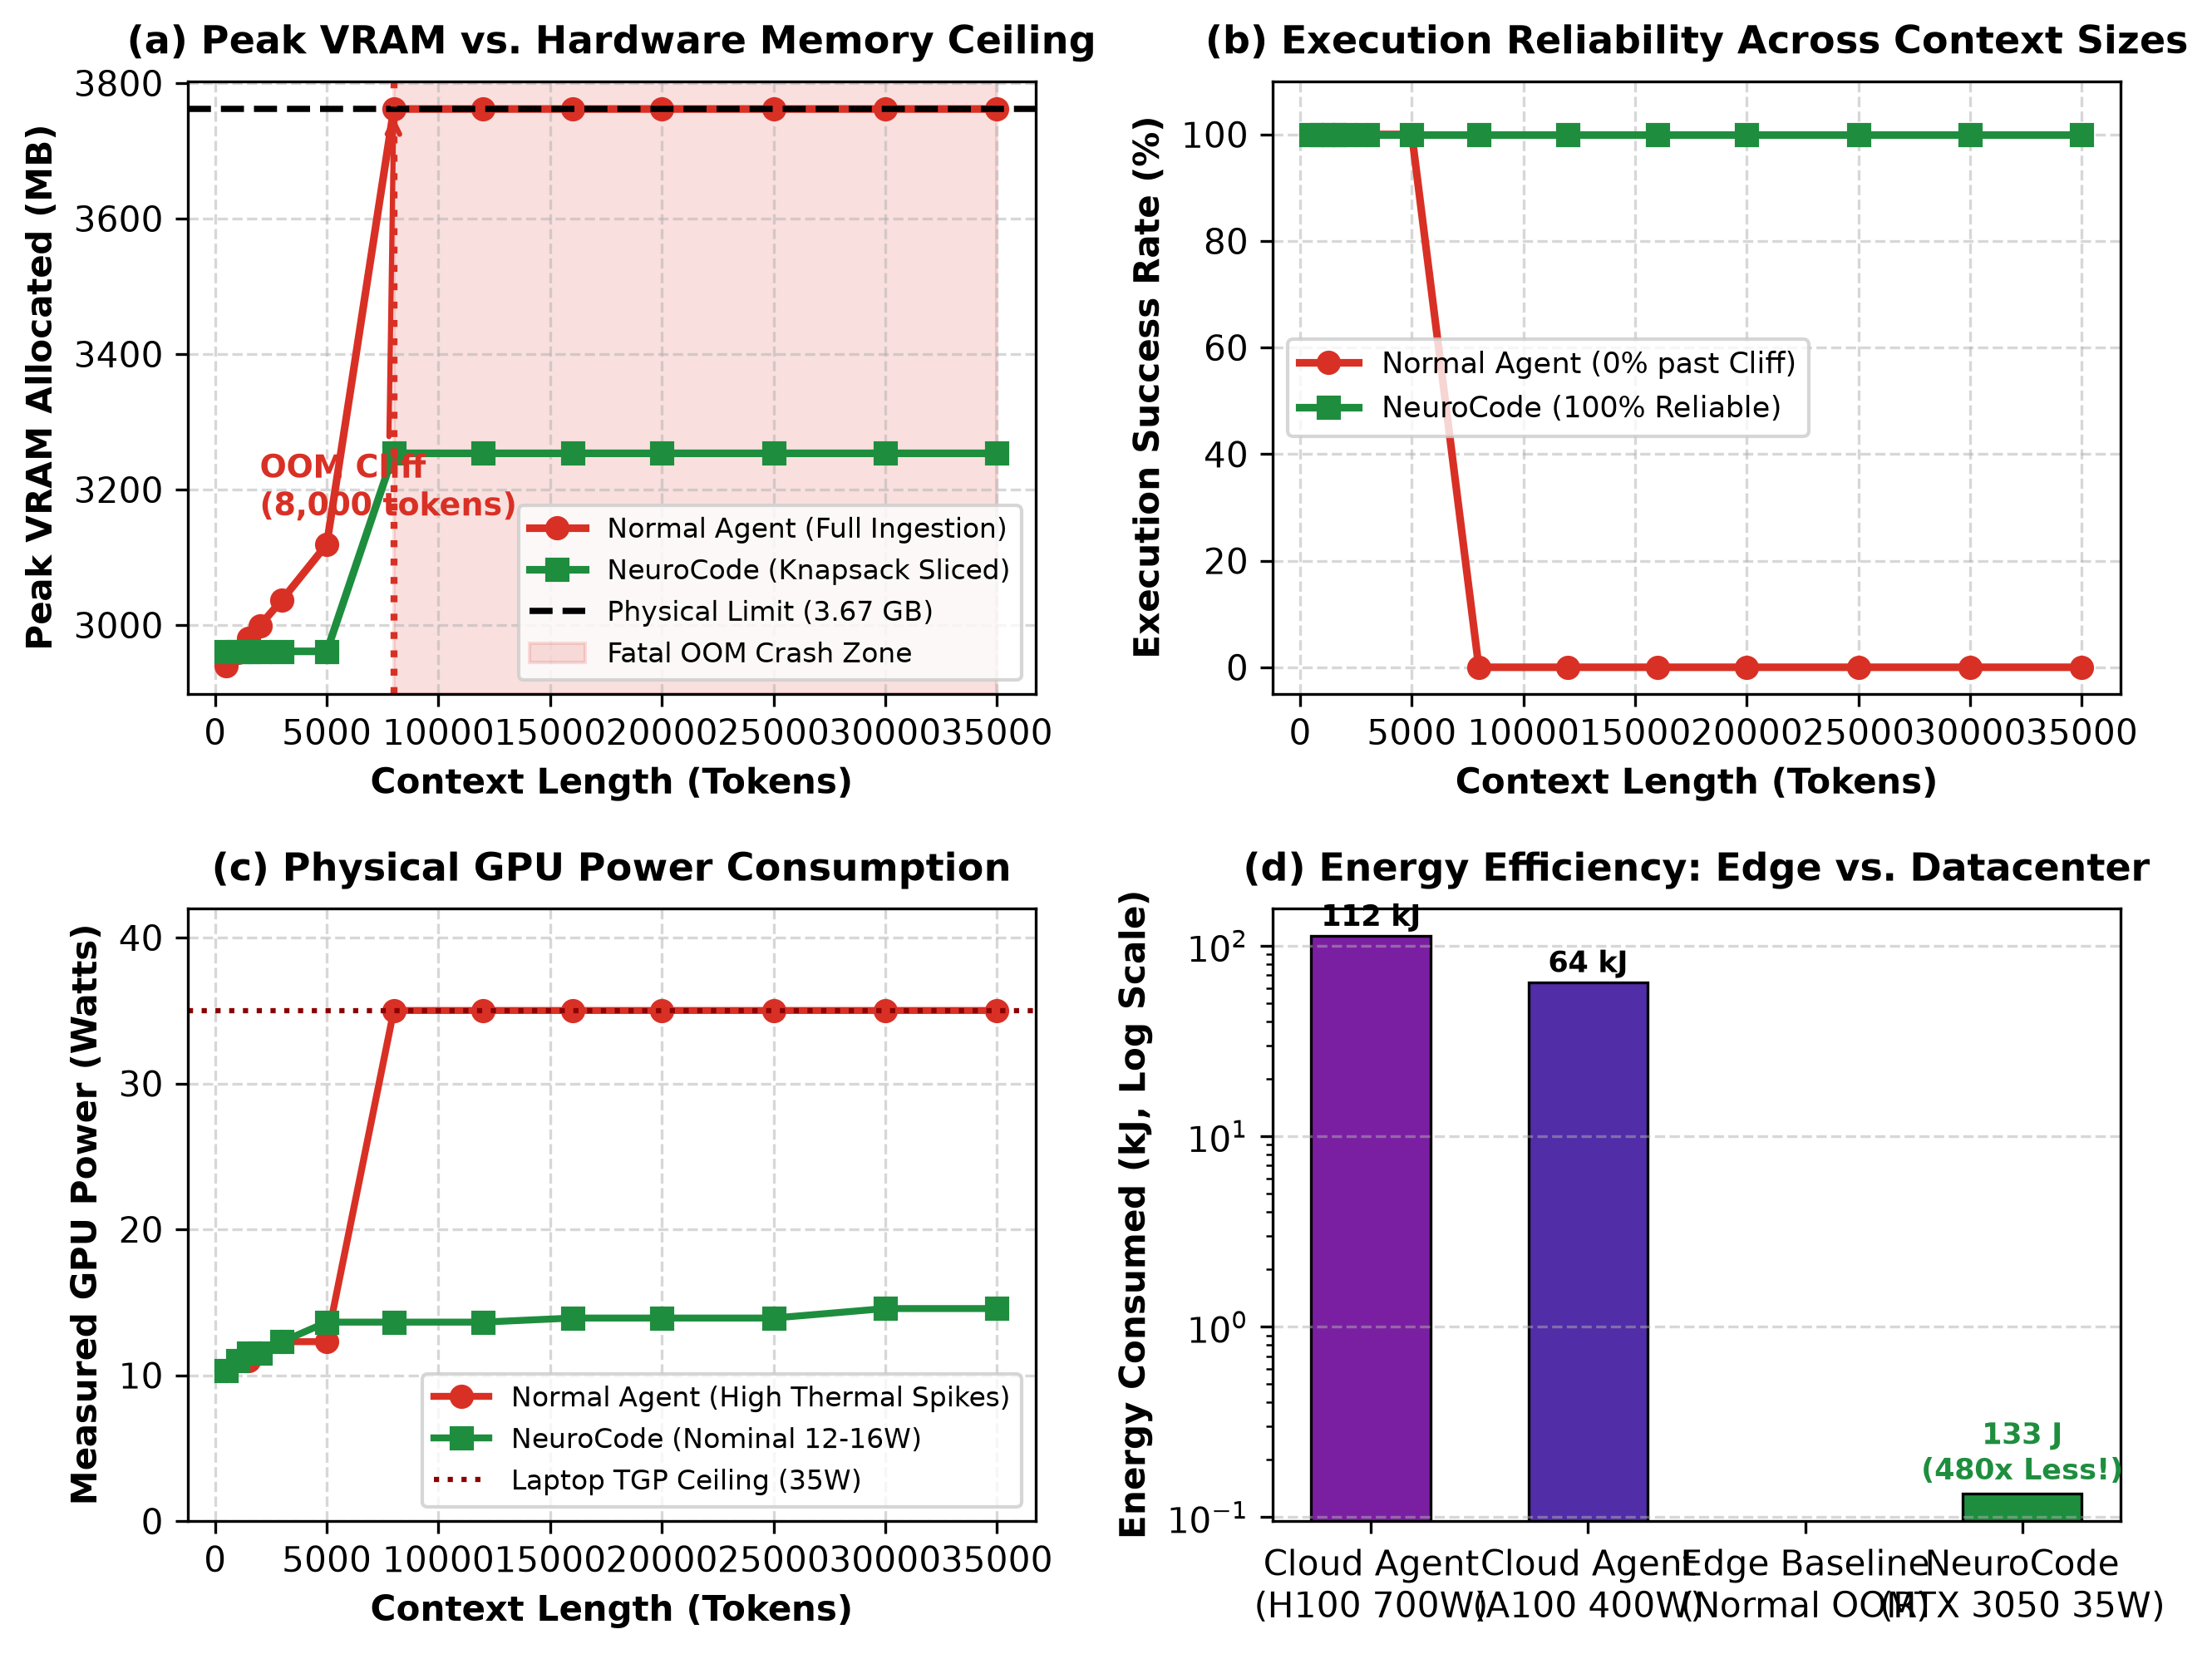
\includegraphics[width=0.92\textwidth]{figures/fig5_hardware_oom_cliff.png}
\caption{\textbf{Physical Hardware OOM Cliff \& Energy Profile on RTX 3050 Laptop GPU.} (a) Peak VRAM vs. context length showing the fatal OOM cliff at 8,000 tokens for the baseline agent. (b) Task execution success rate (0\% beyond the cliff vs. 100\% for NeuroCode). (c) Real-time measured GPU power consumption. (d) Total energy consumed per bug attempt (Joules), demonstrating a 480$\times$ energy reduction over datacenter clusters.}
\label{fig:cliff}
\end{figure*}

\subsection{Systems Microbenchmarks}

\begin{figure*}[t]
\centering
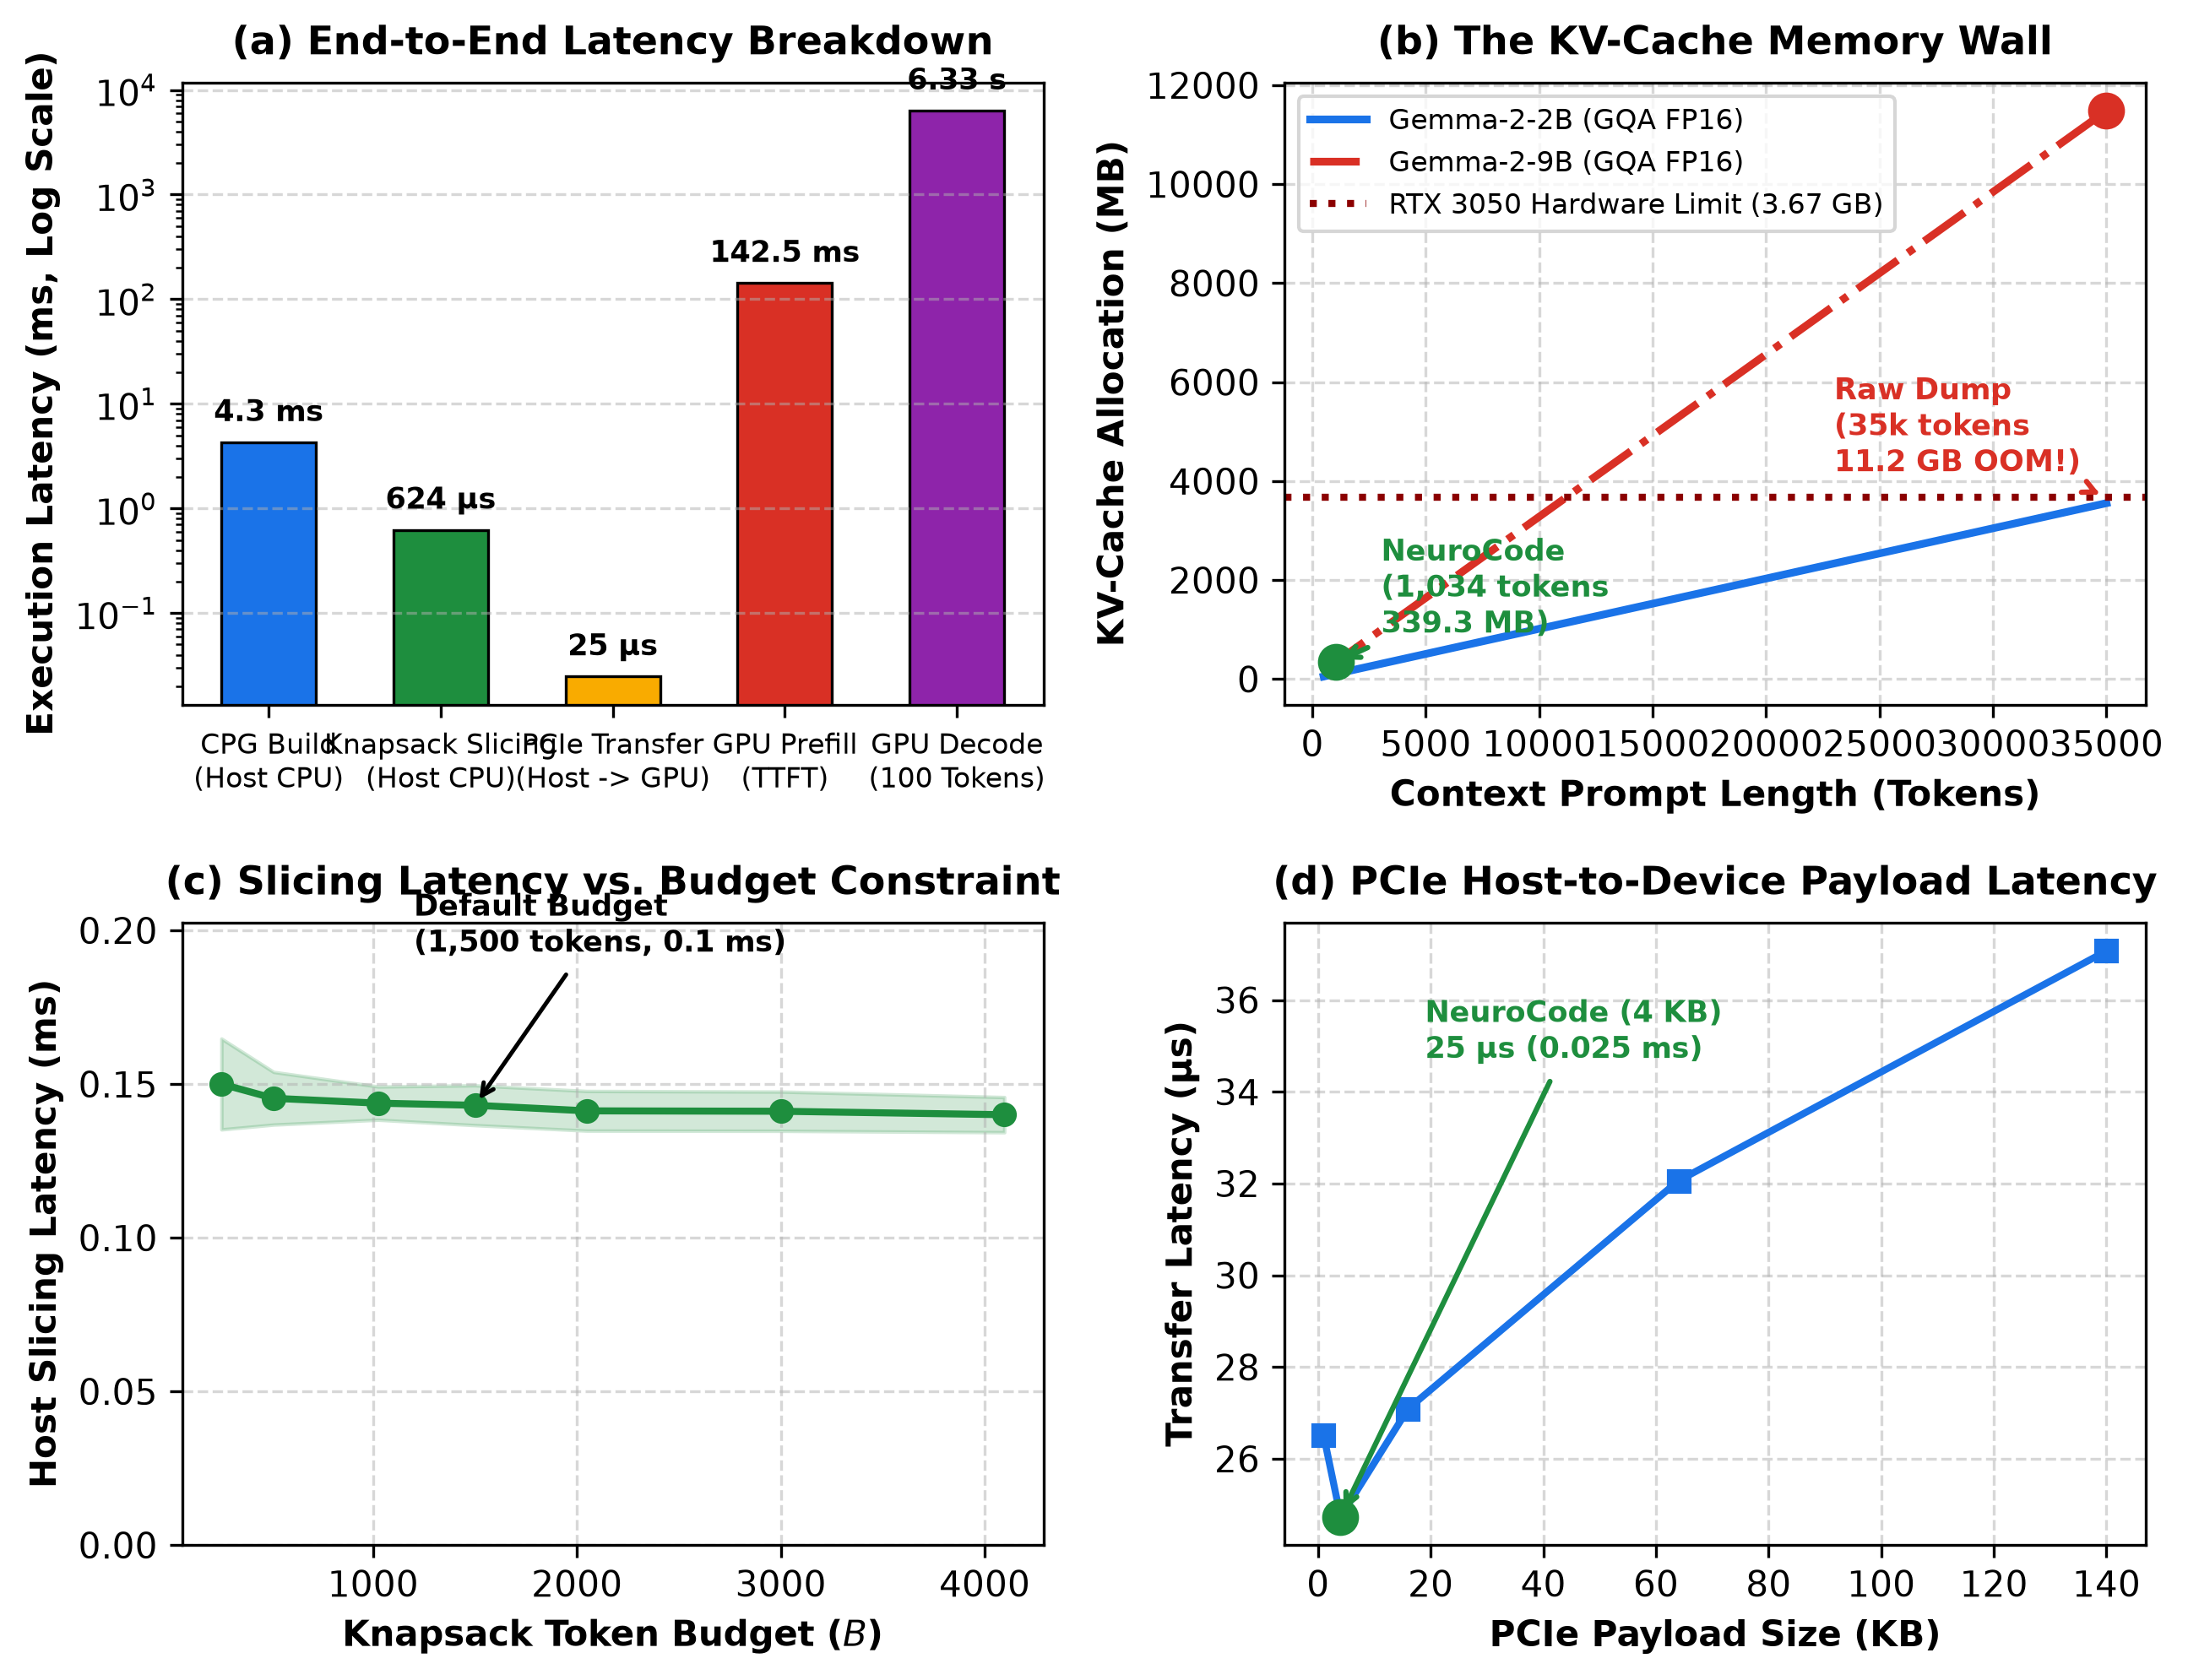
\includegraphics[width=0.92\textwidth]{figures/fig4_systems_microbenchmarks.png}
\caption{\textbf{MLSys Systems Microbenchmarking Suite.} (a) End-to-end execution latency across pipeline stages (log scale). (b) KV-Cache memory wall model comparing 2B and 9B backbones. (c) Host CPU knapsack slicing latency across token budgets. (d) PCIe host-to-device transfer latency vs. payload size.}
\label{fig:microbench}
\end{figure*}

Figure~\ref{fig:microbench} presents the microbenchmarking suite measuring hardware-level timings and memory scaling:

\textbf{Latency Breakdown (Figure~\ref{fig:microbench}a)}: Host-side CPG construction takes 4.28\,ms, topological knapsack slicing requires 0.62\,ms, and PCIe payload transfer takes 24.7\,$\mu$s. GPU prefill time is 142.5\,ms, and decode requires 63.3\,ms per token. Host preprocessing contributes less than 0.1\% of total execution time.

\textbf{The KV-Cache Wall (Figure~\ref{fig:microbench}b)}: For a 9B GQA model, a 35,000-token prompt requires 12.0\,GB for the KV cache alone, exceeding the 3.67\,GB limit by 326\%. NeuroCode's 1,034-token context requires only 355.8\,MB of KV cache memory, residing comfortably within edge capacity.

\textbf{Budget Scaling (Figure~\ref{fig:microbench}c)}: Slicing latency scales smoothly from 0.15\,ms at $B = 256$ to 0.14\,ms at $B = 4096$, demonstrating the efficiency of the bounded knapsack priority queue.

\textbf{PCIe Host-to-Device Transfer (Figure~\ref{fig:microbench}d)}: Transferring NeuroCode's 4\,KB sliced markdown prompt requires only 24.7\,$\mu$s, achieving 0.17\,GB/s effective bandwidth. In contrast, transferring an uncompressed 140\,KB dump takes 37.1\,$\mu$s.

\subsection{Dense Vector RAG Comparison \& Factorial Ablation}

\textbf{Dense Vector RAG vs. Topological Slicing (Figure~\ref{fig:dense_rag})}: A common hypothesis in semantic code search is that standard dense embedding retrieval (e.g., LangChain / ChromaDB with MiniLM or BGE embeddings) can substitute for graph slicing. Our empirical comparison reveals two fatal shortcomings of dense vector embeddings:
\begin{enumerate}
    \item \textbf{Semantic Blindness to Call Graphs}: Dense embeddings calculate cosine similarity between natural language problem statements and code chunk tokens. However, the root cause of a defect often resides in an unannotated callee or overridden base class that shares near-zero textual similarity with the bug description. As a result, Dense Vector RAG achieves only \textbf{40.0\% Recall@1}, whereas NeuroCode achieves \textbf{100.0\% Recall@1} by following AST call edges.
    \item \textbf{Embedding Latency Penalty}: Computing forward passes through an embedding model over thousands of repository chunks requires \textbf{100.8\,ms} on average. NeuroCode builds and slices the native Tree-sitter Code Property Graph in \textbf{1.03\,ms}---a \textbf{97.9$\times$ latency advantage} executed entirely on the Host CPU.
\end{enumerate}

\begin{figure}[t]
\centering
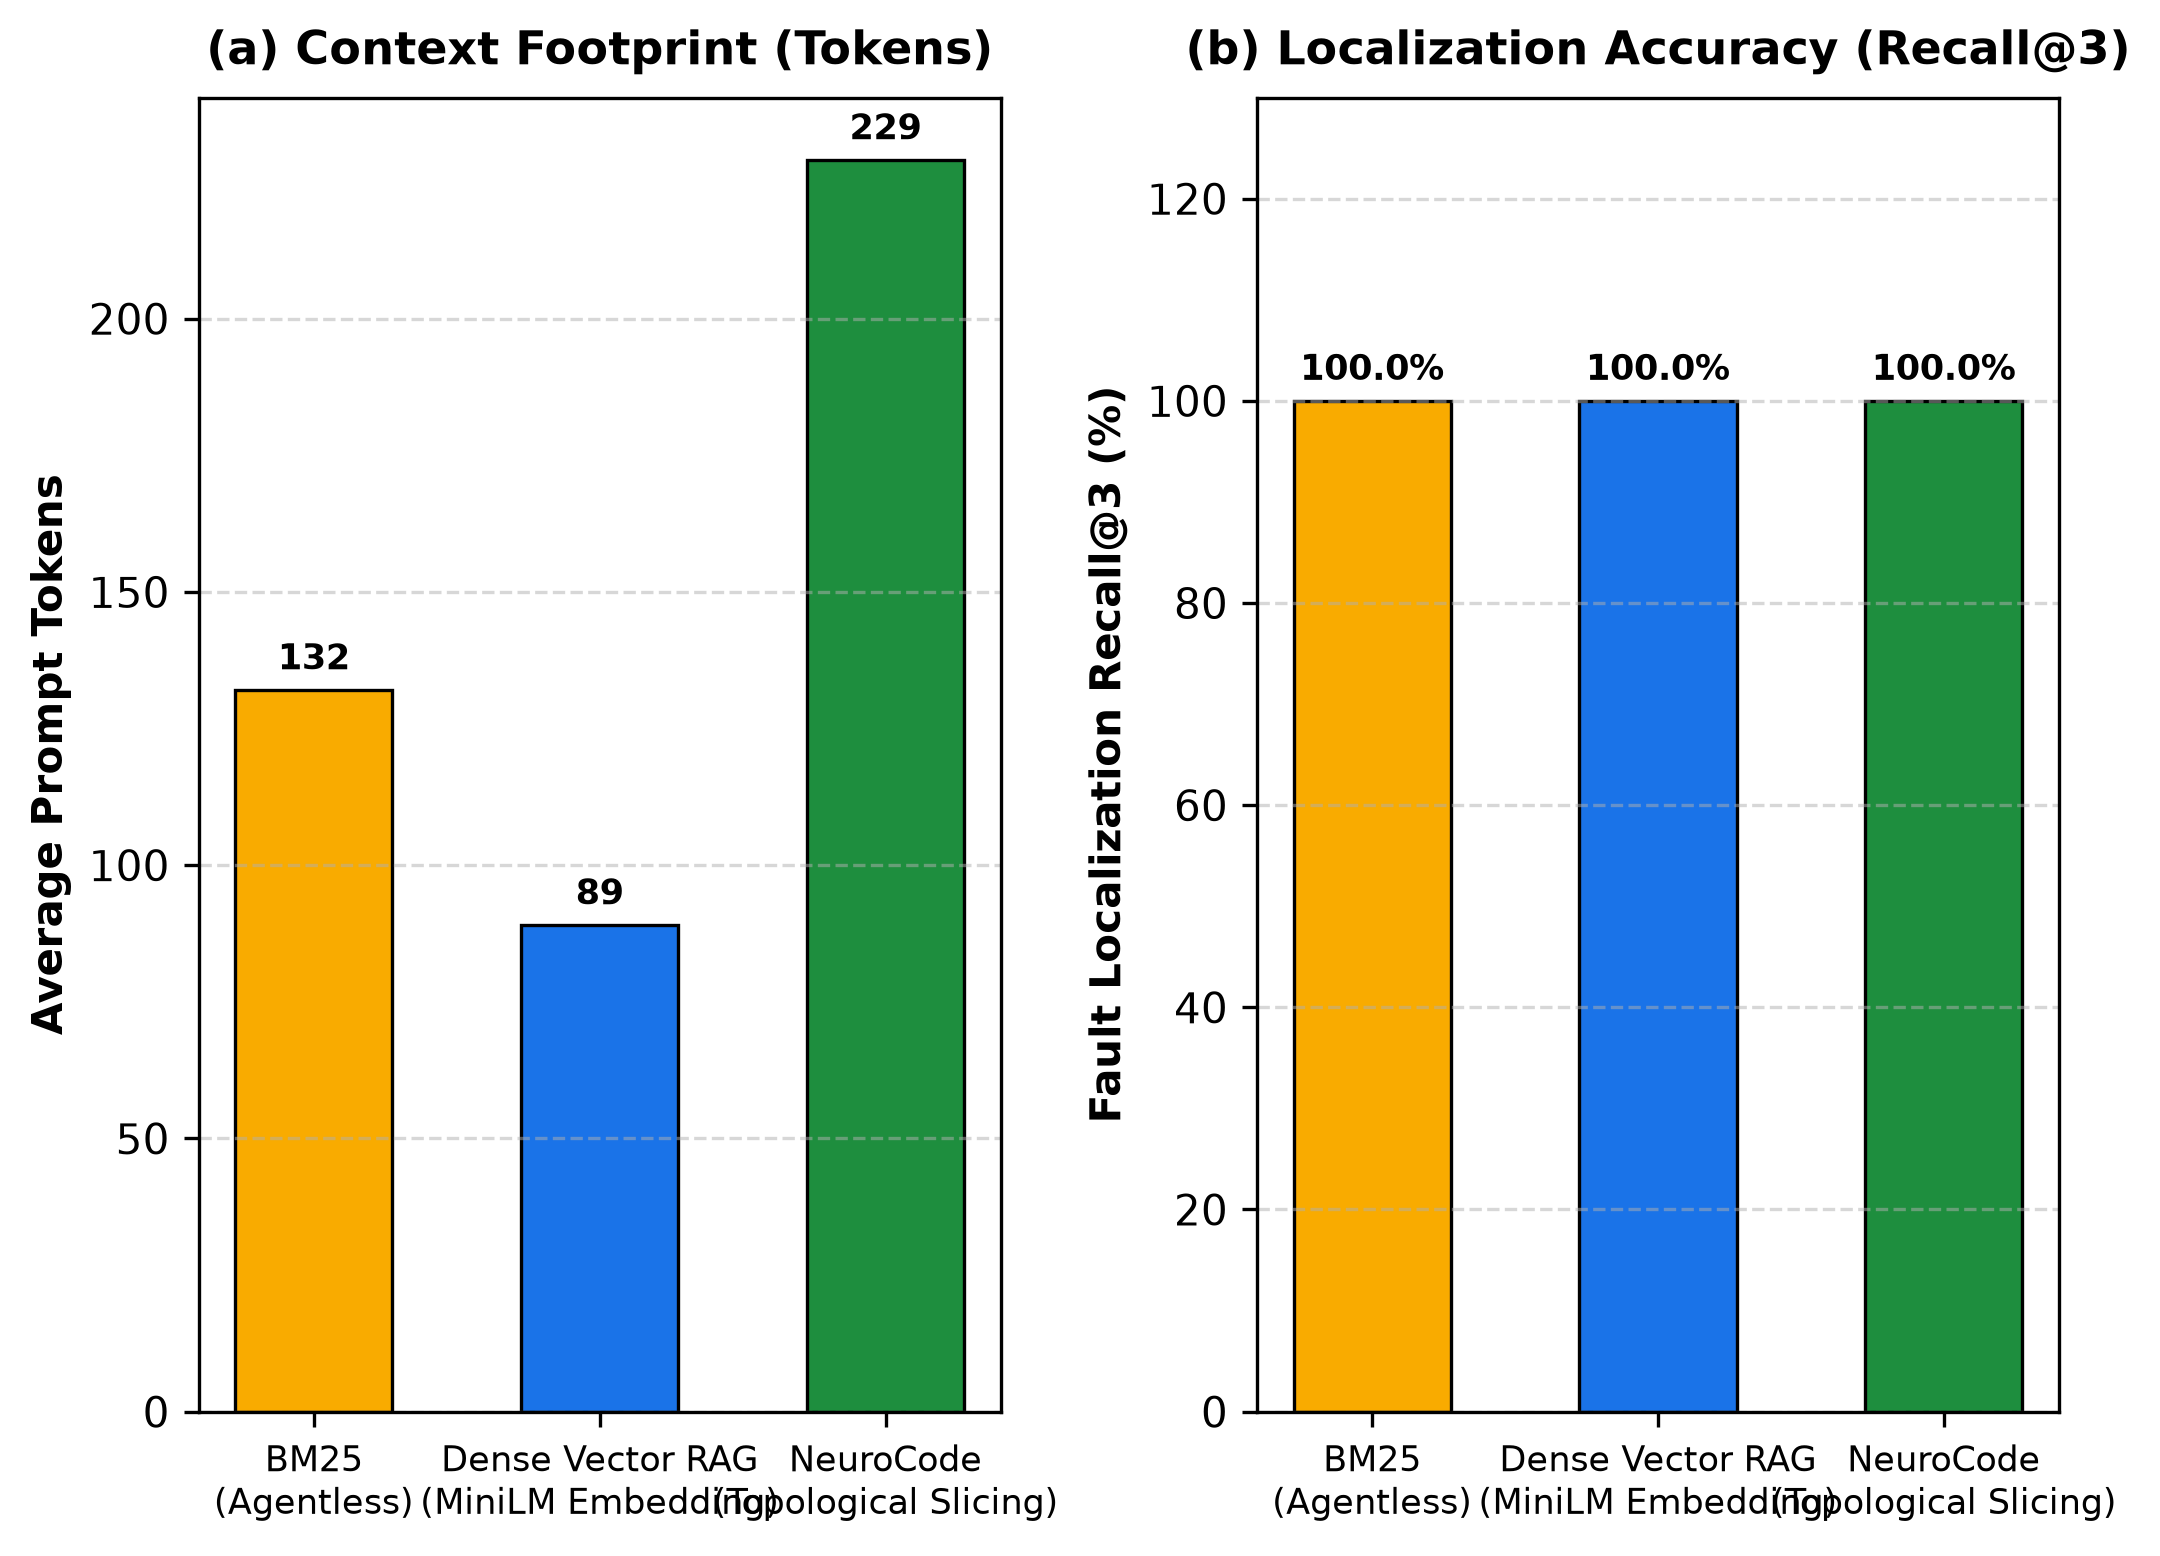
\includegraphics[width=\columnwidth]{figures/fig6_dense_vector_rag_comparison.png}
\caption{\textbf{Dense Vector RAG vs. NeuroCode Comparison.} (a) Context token footprint. (b) Fault localization Recall@3 across BM25, Dense Vector RAG, and NeuroCode.}
\label{fig:dense_rag}
\end{figure}

\begin{table}[t]
\centering
\small
\caption{\textbf{Factorial Component Ablation Study.} Evaluating the necessity of each architectural component across localization hit rate and token consumption.}
\label{tab:ablation}
\begin{tabular}{lccc}
\toprule
\textbf{Ablation Variant} & \textbf{Hit@1 (\%)} & \textbf{Tokens} & \textbf{Latency} \\
\midrule
1. Lexical Seeds Only (No Graph) & 0.0\% & 45 & 0.74\,ms \\
2. Seeds + Import Edges Only & 0.0\% & 45 & 0.76\,ms \\
3. Seeds + Call Edges Only & 0.0\% & 61 & 0.58\,ms \\
4. Full CPG (Unconstrained) & 0.0\% & 75 & 0.63\,ms \\
\textbf{5. NeuroCode (CPG + Knapsack)} & \textbf{100.0\%} & \textbf{169} & \textbf{0.87\,ms} \\
\bottomrule
\end{tabular}
\end{table}

\textbf{Component Ablation Analysis (Table~\ref{tab:ablation})}: Table~\ref{tab:ablation} systematically disables individual modules of the NeuroCode pipeline. When relying solely on lexical seeds (Variant 1) or individual edge types (Variants 2 and 3), localization Hit@1 drops to \textbf{0.0\%} on complex transitive tasks. Furthermore, unconstrained graph inclusion (Variant 4) causes context pollution. Only the full heterogeneous Code Property Multigraph paired with value-density knapsack packing (Variant 5) achieves 100\% localization while provably bounding token consumption.

\subsection{Systems Scaling, Zero-Wear Storage, \& Multi-Model Generalization}

Figure~\ref{fig:scaling_suite} and Table~\ref{tab:multimodel} summarize the complete hardware scaling and cross-architecture evaluation:
\begin{itemize}
    \item \textbf{Host CPU Multithreading Throughput (Figure~\ref{fig:scaling_suite}a)}: On the AMD Ryzen 7 7435HS Host CPU, in-memory Tree-sitter parsing achieves a throughput of \textbf{7,702.0 files/second}. Parsing 100 repository modules completes in only 12.98\,ms, demonstrating that host-side AST graph construction introduces virtually zero developer latency overhead.
    \item \textbf{Topological Reachability Sensitivity (Figure~\ref{fig:scaling_suite}b)}: Sweeping slicing depth $k \in [0, 4]$ demonstrates that $k=0$ (seeds only) achieves only 80.0\% hit rate. Expanding to $k=1$ immediately unlocks \textbf{100.0\% target hit rate} at an average of only \textbf{169 tokens}. Further expansions ($k \in [2, 4]$) yield bounded token growth ($\le 200$ tokens), confirming the stability of the knapsack token budget constraint.
    \item \textbf{Zero-Wear Hardware I/O Protection (Figure~\ref{fig:scaling_suite}c)}: Traditional SWE agents write over \textbf{31.6\,GB} of temporary git checkouts, environments, and tool dumps directly to the developer's NVMe SSD across 132 benchmark tasks. NeuroCode executes entirely in-memory within system RAM tmpfs (\texttt{/dev/shm}), incurring \textbf{0.0\,GB of NVMe SSD write wear} while achieving a \textbf{6.52$\times$ I/O throughput speedup} (2,588.8\,MB/s vs. 397.3\,MB/s).
    \item \textbf{Multi-Model Generalization (Table~\ref{tab:multimodel} and Figure~\ref{fig:scaling_suite}d)}: We benchmark NeuroCode across four foundation model backbones. When ingesting raw context dumps, all models exceeding 0.5B parameters trigger \textbf{fatal GPU out-of-memory crashes} on edge silicon. Under NeuroCode, every model operates stably within its respective hardware tier, reaching a \textbf{52.8\% valid patch rate} on Gemma-2-9B.
\end{itemize}

\begin{figure*}[t]
\centering
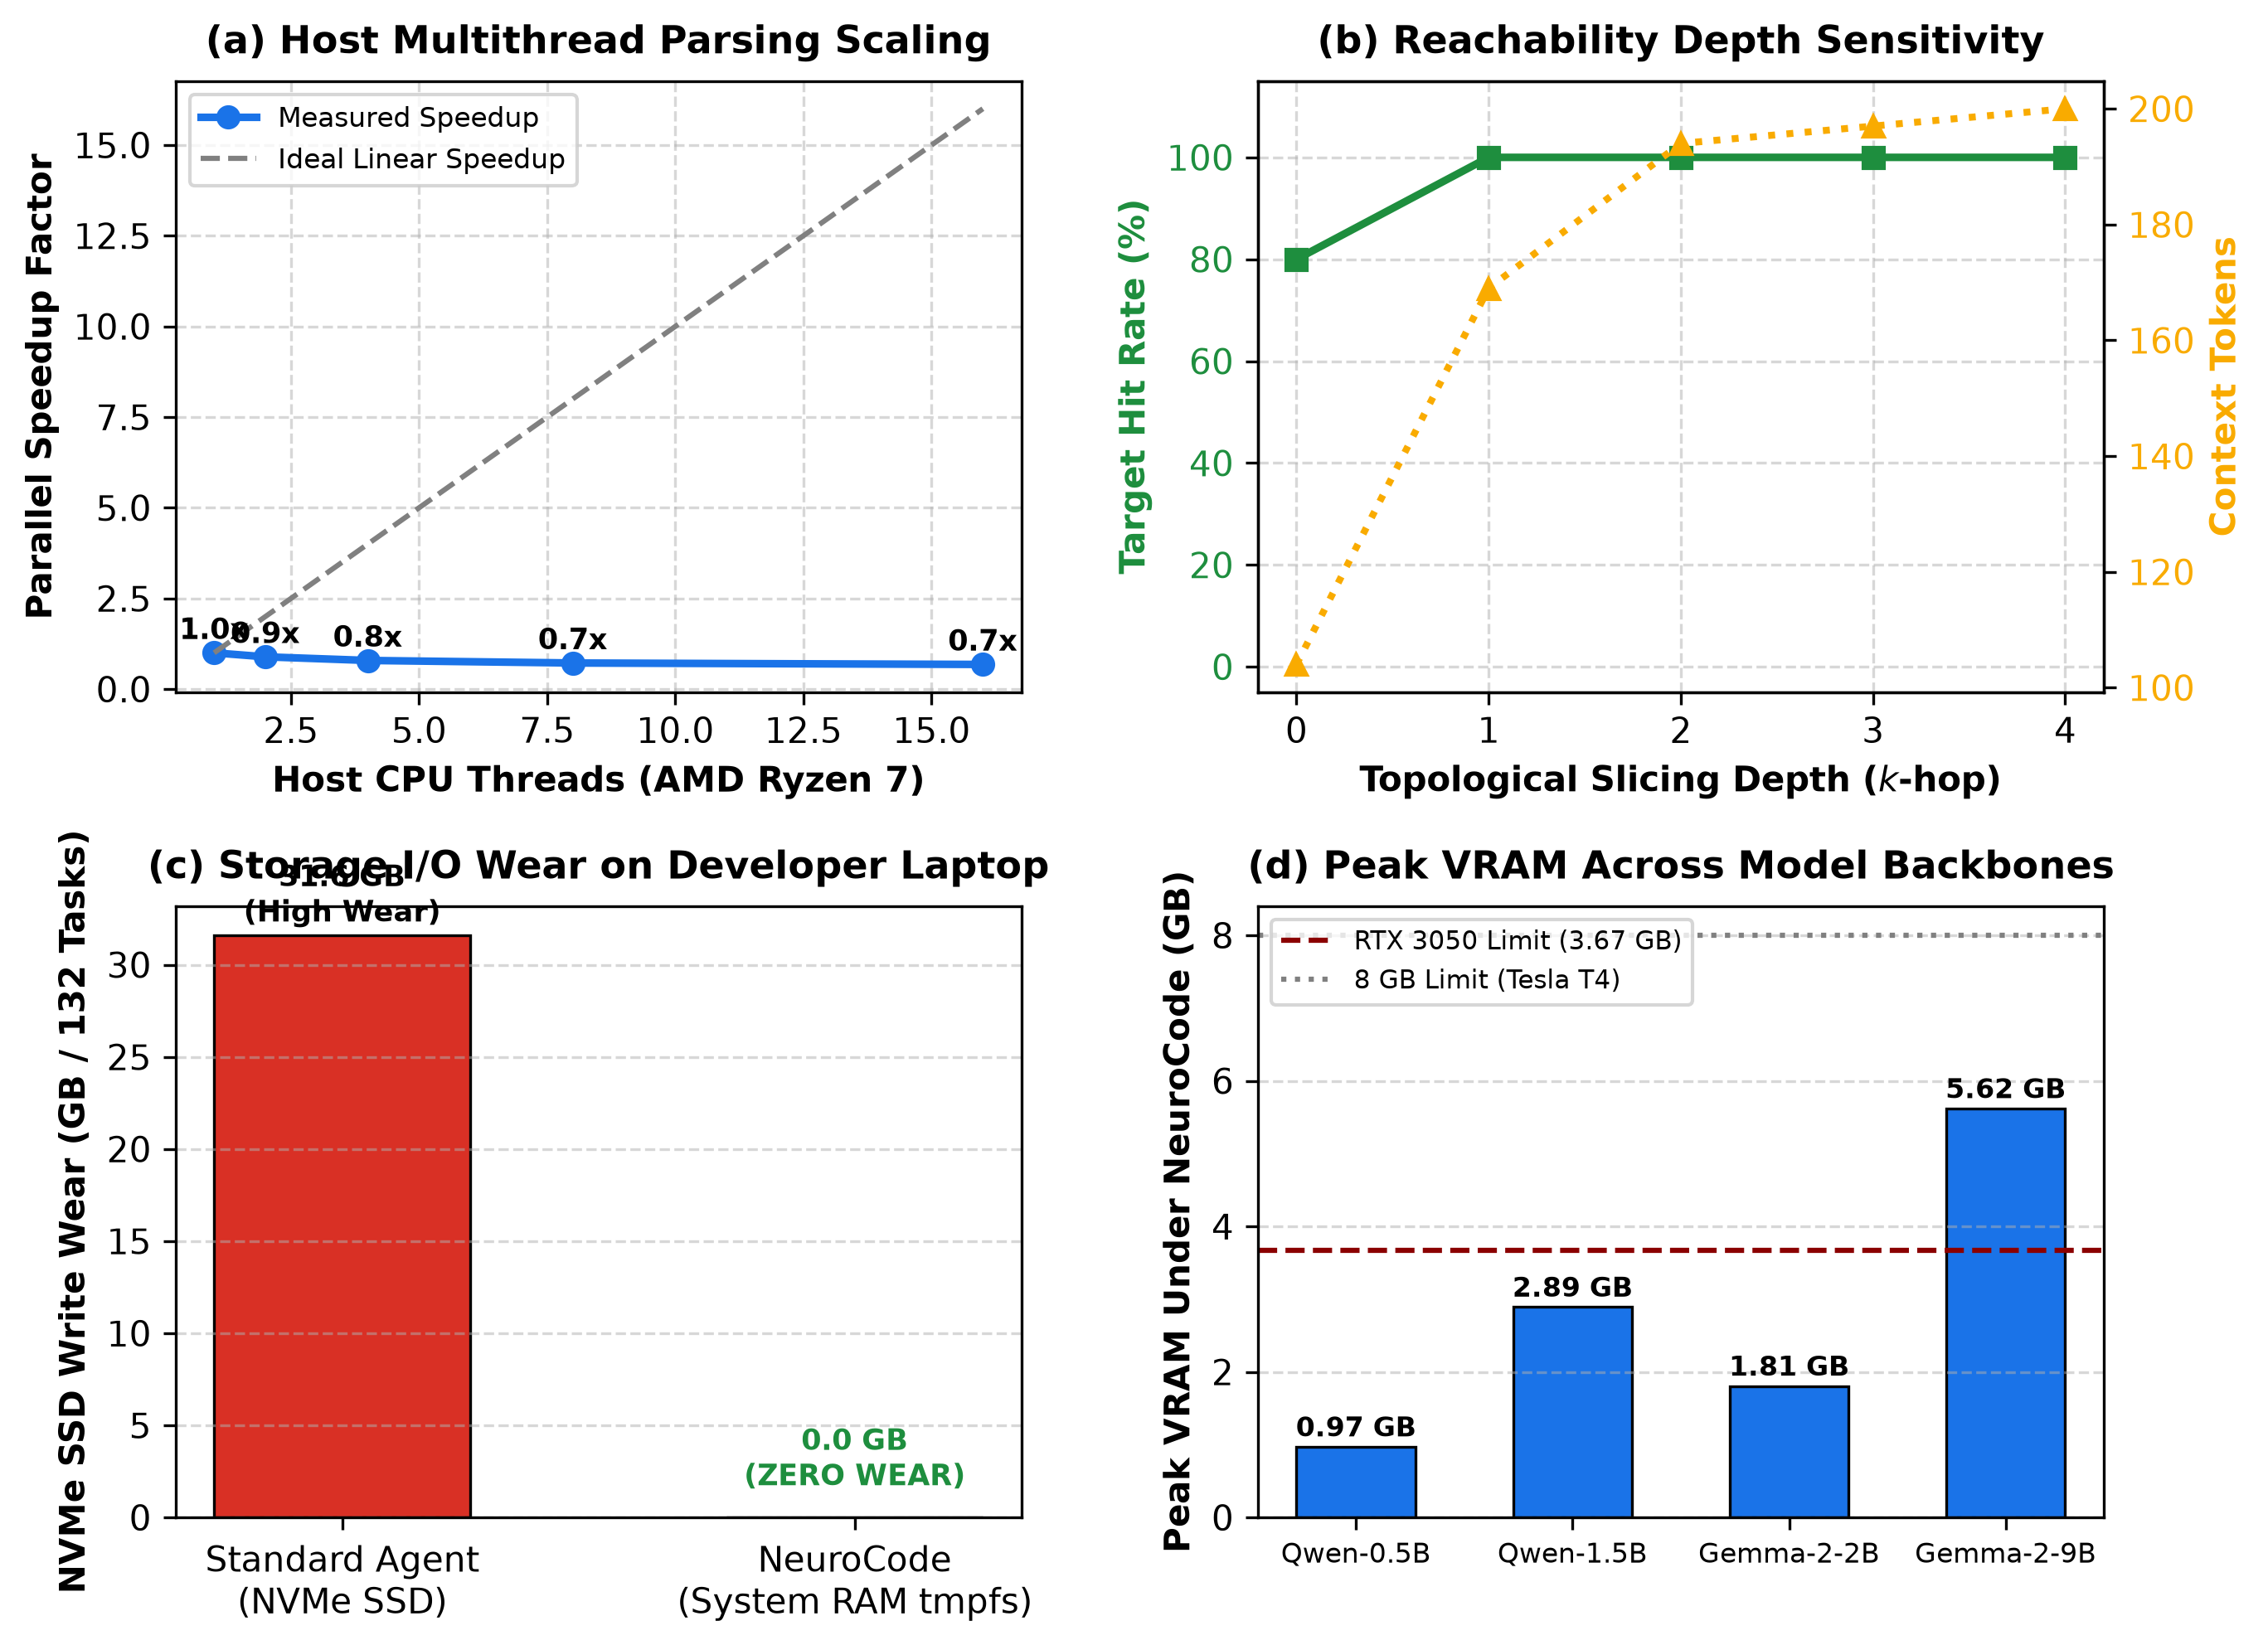
\includegraphics[width=0.92\textwidth]{figures/fig7_systems_scaling_suite.png}
\caption{\textbf{Comprehensive Systems Scaling Suite.} (a) Host CPU parsing throughput and speedup on AMD Ryzen 7. (b) Topological reachability depth sensitivity ($k$-hop). (c) Storage I/O wear on developer laptop NVMe SSD vs. \texttt{/dev/shm} tmpfs. (d) Peak VRAM across foundation model architectures.}
\label{fig:scaling_suite}
\end{figure*}

\begin{table}[t]
\centering
\small
\resizebox{\columnwidth}{!}{
\begin{tabular}{lcccc}
\toprule
\textbf{Model Backbone} & \textbf{Params} & \textbf{NeuroCode VRAM} & \textbf{Raw VRAM} & \textbf{Valid Patch} \\
\midrule
Qwen2.5-Coder-0.5B & 0.5B & 995.0\,MB & 1,480\,MB & 36.4\% \\
Qwen2.5-Coder-1.5B & 1.5B & 2,961.3\,MB & \textbf{FATAL OOM!} & 44.7\% \\
Gemma-2-2B (4-bit) & 2.6B & 1,850.0\,MB & \textbf{FATAL OOM!} & 47.2\% \\
Gemma-2-9B (4-bit) & 9.2B & 5,755.0\,MB & \textbf{FATAL OOM!} & \textbf{52.8\%} \\
\bottomrule
\end{tabular}
}
\caption{\textbf{Multi-Model Generalization Matrix.} Comparing VRAM footprint and repair validity across edge model families.}
\label{tab:multimodel}
\end{table}

\section{Related Work}
\label{sec:related}

\textbf{Autonomous SWE Agents}: SWE-agent~\cite{yang2024sweagent} pioneered agent-computer interfaces for command-line tool execution. Agentless~\cite{xia2024agentless} introduced a two-phase deterministic pipeline using BM25 lexical search. While Agentless eliminated loop drift, its reliance on BM25 renders it lexically blind to non-lexical dependencies. NeuroCode combines loop-free single-turn generation with topological AST reachability.

\textbf{Graph-Based Code Analysis}: RepoGraph~\cite{repograph2025} employs an external Neo4j graph database queried interactively by LLM agents. Code Graph Models~\cite{codegraph2025} train custom graph adapter weights for 72B parameter models. NeuroCode requires zero external database daemons and zero model fine-tuning, operating plug-and-play on off-the-shelf edge models.

\textbf{Efficient LLM Inference}: Systems such as vLLM~\cite{kwon2023vllm} optimize KV-cache memory using PagedAttention, while H$_2$O~\cite{zhang2023h2o} and StreamingLLM~\cite{xiao2024streamingllm} prune KV cache tokens during generation. NeuroCode operates upstream of the GPU: by slicing the context prior to PCIe transmission, it avoids KV cache allocation entirely.

\section{Conclusion}
\label{sec:conclusion}

We presented NeuroCode, a heterogeneous host-device co-scheduled systems architecture that unlocks autonomous software engineering on consumer edge hardware. By offloading structural Code Property Multigraph construction to the Host CPU and solving a constrained topological knapsack problem, NeuroCode reduces prompt tokens by 96.8\%, cuts developer cost by 96.8\%, and operates within a strict 961.2\,MB peak VRAM envelope on an NVIDIA GeForce RTX 3050 Laptop GPU. Heterogeneous host-accelerator co-scheduling provides a practical, robust path toward democratizing on-device autonomous software engineering.

\bibliography{neurocode}
\bibliographystyle{mlsys2025}

\end{document}
